\documentclass{article}
\usepackage[utf8]{inputenc}
\usepackage{graphicx}
\graphicspath{ {./imgs/} }
%\usepackage{apacite}
%\usepackage{bibliographystyle}{apacite}

\usepackage[backend=biber]{biblatex}
\bibliography{bibliografia}
\usepackage{geometry}
\usepackage{indentfirst}
\usepackage[spanish]{babel}
\usepackage{multirow, array} 
\usepackage{amsmath}
\usepackage{amssymb}
\usepackage{hyperref}
\usepackage[nottoc]{tocbibind}
\usepackage{tcolorbox}
\usepackage{listings}
\usepackage{color}
\usepackage{float}
\usepackage{multicol}
\usepackage{pgfplots}
\usepackage[demo]{graphicx}
\usepackage{subfig}
\usepackage{minted}
\newminted{python}{}
\usepackage{verbatim}
\hypersetup{
    colorlinks=true,
    linkcolor=blue,
    filecolor=magenta,      
    urlcolor=cyan,
}
\pgfplotsset{width=10cm,compat=1.9}
\geometry{
 a4paper,
 left=23mm,
 right=23mm,
 top=32mm,
 }
\definecolor{mygreen}{RGB}{28,172,0} 
\definecolor{mylilas}{RGB}{170,55,241}
\lstset{language=Python,
    breaklines=true,%
    keywordstyle=\color{blue},%
    morekeywords=[2]{1}, keywordstyle=[2]{\color{black}},
    identifierstyle=\color{black},%
    stringstyle=\color{mylilas},
    commentstyle=\color{mygreen},%
    showstringspaces=false,%without this there will be a symbol in the places where there is a space
    numbers=left,%
    numberstyle={\small \color{darkgray}},% size of the numbers
    numbersep=0pt, % this defines how far the numbers are from the text
    emph=[1]{for,end,break},emphstyle=[1]\color{red}, %some words to emphasise
    tabsize=4
}
\usepackage[backend=biber]{biblatex}
\addbibresource{bibliografia.bib}

\begin{document}
\pagenumbering{gobble}

%-----------------------------------PORTADA------------------------------------
\vspace{2cm}
\begin{center}
    
\includegraphics[scale=1.6]{logo-unam-bw.jpg}
    \hspace{6cm}
    
\includegraphics[scale=0.29]{imgs/logo-iimas.png}
\end{center}
\vspace{1cm}
\begin{center}
    \textbf{{\Huge Proyecto Final}} 
    \\ \vspace{0.5cm}
    \huge Algoritmo Gen\'etico Aplicado a la Programaci\'on de Horario de Cursos usando Enfoque de Coloreaci\'on de Gr\'aficas  
    \\ \vspace{0.5cm}
    \textit{\Large Computaci\'on Concurrente }
    \\ \vspace{0.5cm}
    \Large I.I.M.A.S.
    \\ \vspace{0.2cm}
    \Large U.N.A.M
    \\ \vspace{1cm}
    \huge Barajas Cervantes Alfonso\\
    \huge Cabello Figueroa Israel\\
    \huge Cerritos Lira Carlos  \\
    \huge Franco López Benito Vicente
    \\ \vspace{1.2cm}
    \Large Dr. \'Oscar Alejandro Esquivel  Flores
    \\ \vspace{1cm}
    \Large 9 de febrero del 2021
\end{center}
%-----------------------------------------CONTENIDO----------------------------------------
\newpage
\pagenumbering{arabic}
\begin{abstract}
    En este  documento presentamos un  diseño, análisis e implementación de un algoritmo gen\'etico para el problema de  coloreo de gr\'aficas. El algoritmo gen\'etico desarrolado aqu\'i utiliza m\'as de una selecci\'on de padre y m\'etodos de mutaci\'on dependiendo en el estado de fitness de la mejor soluci\'on. Esto resulta en un cambio de la soluci\'on al \'optimo global m\'as r\'apidamente que usando una selecci\'on de un padre o el m\'etodo de mutaci\'on. Conseguimos colorear de un noventa a un cien por ciento nuestras gráficas de muestra con el algoritmo con la cantidad de colores requerida para cada problema.
    Así mismo se mejora este programa usando una implementación concurrente de este algoritmo. Presentamos la implementación y comparación del algoritmo paralelo con una versión secuencial. Obtuvimos un rendimiento de tres a seis veces superior para nuestros casos de aplicación con la versión paralela.  

\end{abstract}

%\section{Requerimientos}
%\begin{enumerate}
%    \item{Realizar la investigación correspondiente a los %algoritmos evolutivos y su aplicación}
%    \item{Evaluar,elegir y analizar un algoritmo de interes que pueda ser ejecutado de manera concurrente}
    %\item{Considerar un problema de aplicación del algoritmo evolutivo elegido en el punto anterión}
    %\item{Plantear el problema y hacer el analisis de la implementación concurrente}
    %\item{Elaborar el análisis correspondiente de la implementación considerando
    %\begin{itemize}
    %    \item Validación de resultados
    %    \item Tiempo de ejecución de la implementación secuencial
    %    \item Tiempo de implementación de la ejecución concurrente
    %\end{itemize}}
   
%\end{enumerate}


\section{Algoritmos evolutivos , computación evolutiva y más}

\subsection*{Marco Hist\'orico}

En 1859, Darwin publica su libro El origen de las especies que levantó agrias
polémica en el mundo científico por las revolucionarias teorías que sostenían que las
especies evolucionan acorde al medio, para adaptarse a éste.
De esta manera el universo pasaba de ser una creación de Dios estática y perfecta y
se planteaba como un conjunto de individuos en constante competición y evolución para
poder perpetuar su especie en el tiempo. Las especies se crean, evolucionan y
desaparecen si no se adaptan de forma que solo los mejores, los más aptos, los que
mejor se adapten al medio sobreviven para perpetuar sus aptitudes. 
De acuerdo con esta visión de la evolución, la computación ve en dicho marco un
claro proceso de optimización: se toman los individuos mejores adaptados –mejores
soluciones temporales –, se cruzan –mezclan–, generando nuevos individuos –nuevas
soluciones– que contendrán parte del código genético –información– de sus antecesores,
y el promedio de adaptación de toda la población se mejora.

La computación evolutiva se ha convertido en un concepto general adaptable para
resolución de problemas, en especial problemas difíciles de optimización, ella encuentra fuerza combinada con otras técnicas como lo es la computación concurrente.\cite{Coley (1999)}

\subsection*{Explicación sobre los algortimos evolutivos}

La rama de la \text{computaci\'on evolutiva} es en si una rama que envuelve una gran comunidad de gente, ideas y de aplicaciones. Aunque sus raices genealogicas podemos tenerlos desde 1930, surgi\'o como la emergencia de una relativa tecnologia computacional digital no costosa en la d\'ecada de los 60, que sirvi\'o como un importante catalizador para la rama. La viabilidad de usar esta tecnolog\'ia fue de gran importancia para realizar simulaciones como herramiento para analizar sistemas mucho m\'as complejos que aquellos que se podr\'ian analizar matem\'aticamente.\cite{Coley (1999)}

Los algoritmos genéticos son herramientas que podemos usar aplicando aprendizaje máquina que algunas veces nos permite encontrar soluciones para problemas que podrían tener un número muy grande de potenciales soluciones. Cuando resolvemos un problema con un algoritmo genético en lugar de emplear una solución específica, necesitamos dar carácterísitcas y reglas a la solución para que estás sean aceptadas. Cuando estamos viendo por ejemplo si pensamos en la tarea de llenar un camión de carga, debemos establecer principios y reglas que restringan los posibles ordenes en que acomodemos las cosas, por ejemplo una primera regla podría ser meter las cosas más pesadas primero, las cosas frágiles al final, para colocarlas en sitios donde no se golpeen. Estás reglas restrigen el espacio de posibles soluciones.


Ahora pensemos que estamos resolviendo un problema en particular de adivinar un numero, entre 1 y 1000, y tenemos solo diez opciones para adivinar. Si la única retroalimentación que tienes del número, es si escogiste correctamente, o incorrectamente, entonces tu mejor oportunidad es de 1 en 100 de adivinar el número. Con los algoritmos genéticos recibimos información adicional, dan una retroalimentación acerca de que tan cerca o lejos están de la solución.
Si en lugar de correcto o incorrecto recibimos este indicador, la probabilidad de encontrarlo es total, porque con búsqueda binaria podemos encontrar cualquier número entre 1 y 1000 en diez pasos.



\subsection{Clasificación de los algoritmos evolutivos}
\begin{enumerate}
    \item Estrategias Evolutivas:
Fue diseñada inicialmente
con la meta de resolver problemas de optimización discretos y continuos,
principalmente experimentales y considerados difíciles. Trabaja con vectores de
números reales Dcon desviaciones estándarD que codifican las posibles soluciones de
problemas numéricos. Utiliza recombinación o cruce (crossover aritmético), mutación y
la operación de selección, ya sea determinística o probabilística, elimina las peores
soluciones de la población y no genera copia de aquellos individuos con una aptitud por
debajo de la aptitud promedio.
  \item{Programación Evolutiva:}
  Inicialmente fue diseñada como un intento de crear inteligencia artificial.
La representación del problema se realiza mediante números reales (cualquier estructura
de datos), y emplea los mecanismos de mutación y selección. El procedimiento es muy
similar a las estrategias evolutivas con la diferencia de que no emplea la recombinación,
de tal forma que son denominadas en conjunto algoritmos evolutivos como una manera
de diferenciarlas de los algoritmos genéticos. 
\item{Algoritmos Genéticos:}
Modelan el proceso de evolución como una sucesión de
frecuentes cambios en los genes, con soluciones análogas a cromosomas. Trabajan con
una población de cadenas binarias para la 
 representación del problema, y el espacio de
soluciones posibles es explorado aplicando transformaciones a éstas soluciones
candidatas tal y como se observa en los organismos vivientes: cruce, inversión y
mutación. Como método de selección emplean en mecanismo de la ruleta (a veces con
elitismo). Constituyen el paradigma más completo de la computación evolutiva ya que 
resumen de modo natural todas las ideas fundamentales de dicho enfoque. Son muy
flexibles ya que pueden adoptar con facilidad nuevas ideas, generales o específicas, que
surjan dentro del campo de la computación evolutiva. Además, se pueden hibridar
fácilmente con otros paradigmas y enfoques, aunque no tengan ninguna relación con la
computación evolutiva. Se trata del paradigma con mayor base teórica.\cite{Coley (1999)}
\end{enumerate}
\subsection{Procesos Evolutivos B\'asicos}
Un lugar bueno para empezar es preguntarse los componentes b\'asicos de un sistema evolutivo. La primer nota que debemos tomar en cuenta es que existen al menos dos posibles interpretaciones de un \textit{Sistema Evolutivo}. Es frecuentemente usado para describir un sistema que cambia con incrementos a lo largo del tiempo. La segunda interpretaci\'on es aquella que tiene un sentido biol\'ogico, es decir, que es un sistema evolutivo Darwiniano.\cite{Goldberg(1989)}

Para ello, precisamos saber lo que entendemos por un \textit{Sistema}. Una manera es identificando lo que precisamente constituye al sistema, es decir todas sus partes. A continuaci\'on se presenta el conseso de lo que se entiende por un sisteme evolucionario Darwiniano.
\begin{itemize}
    \item Una o m\'as poblaciones compiten por limitados recursos
    \item Noci\'on de que las poblaciones cambien din\'amicamente debido al nacimiento y la muerte de individuos.
    \item El concepto de la aptitud en donde refleja la habilidad de un individuo de sobrevivir y de reproducirse
    \item El concepto de  herencia variacional: la descendencia se parece mucho a sus padres, pero son no es identicos.
\end{itemize}
\subsection{Un primer ejemplo: Un simple Sistema Evolutivo}
La primera cuestión a afrontar es cómo representar a los individuos (organismos) que componen una población en evolución. Una técnica bastante general es describir a un individuo como un vector de longitud de las características L que se eligen presumiblemente debido a su relevancia (potencial) para estimar la aptitud de un individuo. Entonces, por ejemplo, los individuos podrían caracterizarse por:
\begin{equation*}
    < \textrm{color cabello, color ojos, color piel, altura, peso}>
\end{equation*}
Podríamos pensar libremente en este vector como que especifica la composición genética de un individuo, es decir, su genotipo especificado como un cromosoma con cinco genes cuyos valores dan como resultado un individuo con un conjunto particular de rasgos. Alternativamente, podríamos considerar tales vectores como descripciones de los rasgos físicos observables de los individuos, es decir, su fenotipo. En cualquier caso, por especificando adicionalmente el rango de valores (alelos) que tales características pueden asumir, se define un espacio de cinco dimensiones de todos los posibles genotipos (o fenotipos) que los individuos pueden tener en este mundo artificial.\footnote{El ejemplo fue obtenido de \cite{Cuevas (2016)}}
\begin{verbatim}
EV:
    Generar una poblacion inicial de M individuos
    DO FOREVER:
        Seleccionar un miembro del la actual poblacion para que sea padre
        
        Usa el seleccionado padre para que produzca una descendencia que
        sea similar pero generalmente no una copia precisa del padre
        
        Selecciona a un miembro de la poblacion para que muera
        END DO
\end{verbatim}




\subsection{Algoritmos Evolutivos,investigación}
%\subssubsection*{Travelling salesman problem}
%Given a list of cities and the distances between each pair of cities, what is the shortest possible route that visits each city exactly once and returns to the origin city?
\subsubsection{B\'usqueda Aleatoria}
El m\'etodo de b\'usqueda aleatoria  es el primer m\'etodo que bas\'o su estrategia de optimizaci\'on en un proceso totalmente estioc\'astico. Bajo este m\'etodo, s\'olo una soluci\'on canidato $x^k$ es mantenida durante el proceso de evoluci\'on. En cada iteraci\'on, la soluci\'on cadidato $x^k$ es modificada a\~nadiendo un vector aleatorio $\Delta x$. De esta manera, la nueva soluci\'on candidato es modelada bajo la siguiente expresi\'on:
\begin{equation*}
    x^{k+1} = x^{k} + \Delta x
\end{equation*}
Considerando que la soluci\'on candidato $x^k$ tiene $d$ dimensiones $\left( x_1^k,x_2^k, \cdots, x_d^k\right)$, cada coordenada es modificada $\left( \Delta x = \{ \Delta x_1, \Delta x_2, \cdots, \Delta x_d\} \right)$ mediante una perturbaci\'on aleatoria $\Delta x,$ $\left( i \in [1,2, \dots, d]\right)$ mpde;ada por una distribuci\'on de probabilidad gaussiana $p(\Delta x_i) = N(\mu_i, \sigma_i)$, se considera que $\mu_i = 0$ dado que el valor de $\Delta x_i$ a\~nade una modificaci\'on alrededor de $x_i^k$.\\Una vez calculado $x^k+1$, se prueba si la nueva posición mejora la calidad de la solución candidato anterior $x^k$. De esta manera, si la calidad de $x^k+1$ es mejor que $x^k$, el valor de $x^k+1$ es aceptado como la nueva solución candidato, en caso contrario permanece $x^k$ sin cambio.  Esta prueba puede definirse para un caso de minimización como:
\begin{equation*}
     x^{k+1} = \left \{ \begin{matrix} x^{k+1} & \mbox{si }f(x^{k+1}) < f(x^k)
\\ x^k & \mbox{si }f(x^{k+1}) \geq f(x^k)\end{matrix}\right. 
\end{equation*}
A este criterio de sustitución, de aceptar solamente los cambios que mejoren la calidad de la solución es conocido como “\textit{greedy}”. En búsqueda aleatoria, la perturbación $\Delta x$ impuesta a $x^k$ podría hacer que el nuevo valor $x^{k+1}$ quede fuera del espacio de búsqueda denido $X$. Fuera del espacio de búsqueda $X$ no existe denición de la función objetivo  $f(x)$. Para evitar este problema, el algoritmo debe proteger la evolución de la solución candidato $x^k$, de tal forma que si $x^{k+1}$ queda fuera del espacio de búsqueda $X$, se le debe de asignar una muy mala calidad (representado por u valor muy grande). Esto es $f(x^{k+1}) = \infty$ para el caso de la minimizaci\'on o $f(x^{k+1}) = - \infty$ para el caso de la maximizaci\'on.
\cite{Cuevas (2016)}
\begin{figure}[h!]
    \centering
    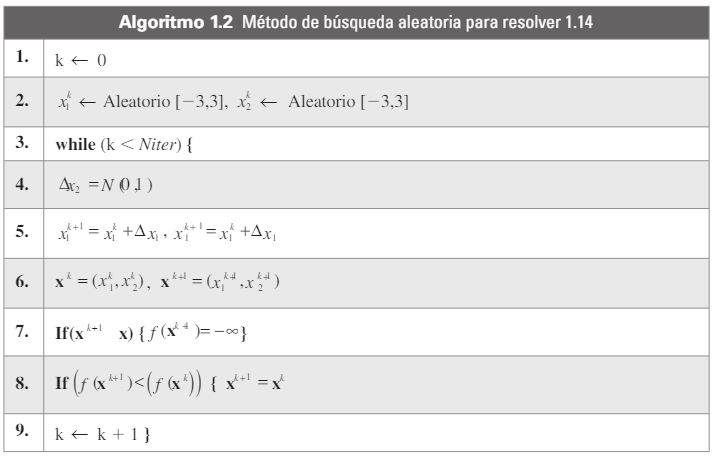
\includegraphics[width=15cm]{imgs/busqueda_aleatoria.JPG}
    \caption{Algoritmo de B\'usqueda Aleatoria}
    \label{fig:my_label}
\end{figure}

\subsubsection{Temple Simulado}
El temple simulado o en ingl\'es 'Simulated annealing' es una t\'ecnica de optimizaci\'on que emula el proceso de templado en materiales met\'alicos. La idea del templado es enfriar el material controladamente de tal manera que las estructuras cristalinas puedan orientarse y evitar los defectos en las estructuras met\'alicas. \\ El uso del templado como inspiraci\'on para la formulaci\'on de algoritmos de optimizaci\'on fue por primera vez propuesto por Kirkpatrick, Gelatt y Vecchi en 1983. Desde entonces se han sugerido varios estudios y aplicaciones para analizar los alcances del m\'etodo.A diferencia de algoritmos basados en gradiente, el m\'etodo del temple simulado presenta una gran habilidad para evitar quedar atrapados en los m\'inimos locales.\\En el templado simulado, el valor de la función objetivo que se intenta optimizar es análogo a la energía de un sistema termodinámico. En altas temperaturas el algoritmo permite la exploración de puntos muy distantes entre sí en el espacio de búsqueda, además de que la probabilidad de aceptación de soluciones que no mejoran su estado anterior es muy grande. Po el contrario, a bajas temperaturas, el algoritmo permite \'unicamente la generaci\'on de puntos muy cercanos entre s\'i, adem\'as de que la probabildiad de aceptaci\'on se reduce, por lo que ahora s\'olo las nuevas soluciones que mejoren su estado anterior, ser\'an consideradas.\\El \textit{algoritmo de temple simulado} matiene urante su funcionamiento una sola soluci\'on candidato $(x^k)$. Dicha soluci\'on es modificada en cada iteraci\'on utilizando un procedimiento similar al de m\'etodo de b\'usqueda aleatoria, donde cada punto es modificado mediante la generaci\'on de un vector aleatorio $\Delta x$. Sin embargo, este algoritmo no solo acepta los cambios que mejoren su funci\'on objetivo, sino que incorpora un mecanismo probabil\'istico, que le permite aceptar incluso soluciones que le empeoren. Esto con el fin de salir de los m\'inimos locales.
\cite{Cuevas(2016)}
Bajo estas circunstancias, una nueva soluci\'on ser\'a aceptada $x^{k+1}$ considerando dos diferentes alternativas
\begin{itemize}
    \item Si su calidad es superior a la de su antecesor $x^k$. Esto es si $f(x^{k+1})>f(x^k)$
    \item Bajo una probabilidad de aceptaci\'on $p_a = e^{\frac{\Delta f}{T}}$, donde $T$ representa la temperatura que controla el proceso de templado, mientras que $f$ es la diferencia de energ\'ia entre el puntos $\Delta f= f(x^{k+1})-f(x^k)$
\end{itemize}
A continuaci\'on mostramos el algoritmo de temple simulado.
\begin{figure}[h!]
    \centering
    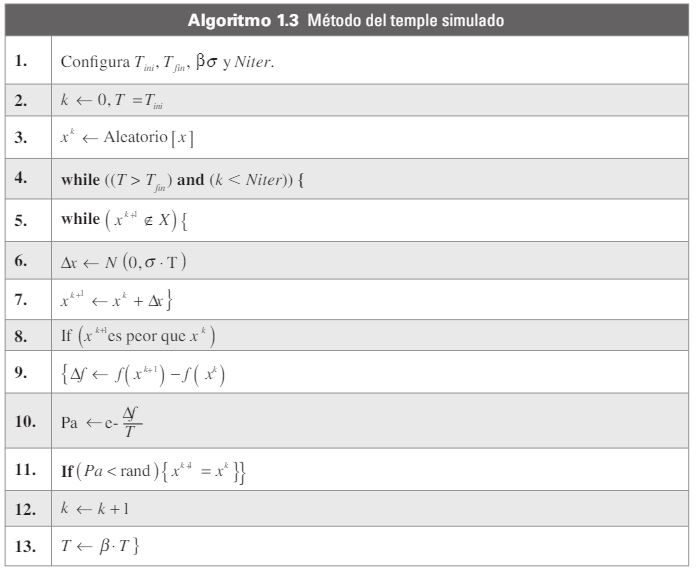
\includegraphics[width=15cm]{imgs/templado_simulado.JPG}
    \caption{Algoritmo de temple simulado}
    \label{fig:my_label}
\end{figure}
\subsubsection{Gen\'eticos}
Un algoritmo genético es un método de búsqueda que imita la
teoría de la evolución biológica de Darwin para la resolución de
problemas. Para ello, se parte de una población inicial de la cual
se seleccionan los individuos más capacitados para luego
reproducirlos y mutarlos para finalmente obtener la siguiente
generación de individuos que estarán más adaptados que la
anterior generación.
\cite{D.Gutierrez,A.  Tapia,2020}
\subsubsection{Implementación}
Una premisa es conseguir que el tamaño de la población sea lo
suficientemente grande para garantizar la diversidad de
soluciones.
Los pasos básicos de un algoritmo genético son:
\begin{itemize}
\item Evaluar la puntuación de cada uno de los cromosomas
generados.
\item Permitir la reproducción de los cromosomas siendo los
más aptos los que tengan más probabilidad de
reproducirse.
\item Con cierta probabilidad de mutación, mutar un gen del
nuevo individuo generado.
\item Organizar la nueva población
\end{itemize}
Se puede fijar un número máximo de iteraciones
antes de finalizar el algoritmo genético o detenerlo cuando no se
produzcan más cambios en la población.

Parametros de los algoritmos geneticos.
\begin{itemize}
    \item Tamaño de la población.
    \item Probabilidad de cruce.
    \item Probabilidad de mutación.
\end{itemize}

Al igual que en otros algoritmos metaheurísticos, los AG presentan algunas ventajas respecto a los métodos clásicos de optimización; por ejemplo, pueden trabajar con poca o ninguna información acerca de la función objetivo, y por ser poblacionales tienen mayores probabilidades de escapar de óp-timos locales, en comparación con los métodos determinísticos. Sin embargo, entre sus desventajas está el hecho de que no garantizan una convergencia al óptimo real, y en muchos casos son más tardados que las técnicas deterministas

\subsubsubsection{Un ejemplo}
Veamos como aplicar un algoritmo genetico para minimizar la siguiente función \footnote{El algoritmo y ejemplo fueron obtenidos de \cite{Cuevas(2016)}}. la cual es dificil desde el punto de vista computacional, pues contiene bastantes optimos locales 
\begin{align*}
    f(x_1,x_2)=a+exp(1)-a*exp(-b\sqrt{\frac{1}{d}(x_1^2+x_2^2)})-exp(\frac{1}{d}(\cos{c_1x_1}+\cos{c_2x_2})) \\
    x_1,x_2 \in [-15,30]
\end{align*}

\begin{verbatim}
    function [temp, ind] = FUNCION(x, d, N) y=[];% 
    Ackley
    for j=1:N       
       a = 20; b = 0.2; c = 2*pi;   
       s1 = 0; s2 = 0;    
       for i=1:d;        
          s1 = s1+x(j,i)^2;       
          s2 = s2+cos(c*x(j,i));   
    end
    y(j,1) = -a*exp(-b*sqrt(1/d*s1))-exp(1/d*s2)+a+exp(1);
    end
    [temp,ind]=sort(y);
\end{verbatim}

Básicamente un AG es un programa que genera una población inicial aleatoria de padres, y durante cada generación selecciona pares de padres, considerando su valor de $f(x_i,)$, para realizar intercambios de material genético, o cruza, y generar pares de hijos; tales hijos serán mutados con una cierta probabilidad, y nalmente competirán por sobrevivir a la siguiente generación con los padres, proceso que se conoce como elitismo. Aunque dicho comportamiento produce la convergencia del algoritmo, también es cierto que provoca que la población sea ‘arrastrada’ por el mejor individuo de la población, lo que conduce en ocasiones un estancamiento de la población

La desventaja de esto es que podria llegarse encontrar un optimo local en ves de uno global

\subsubsection{Estrategias Evolutivas}

Las EE son algoritmos inspirados en la evolución y al igual que otros basados en tal metáfora, sus individuos realizarán una “evolución”, o mejora, con respecto a alguna función objetivo y mediante operadores que imitan dicho proceso.

Podriamos por ejemplo considerar minimizar $f$ tal que:
\begin{align*}
   f(x_1,x_2)=-sen(x1)sen^{2m}(\frac{x_1^2}{\pi})+sen(x_2)sen^{2m}(\frac{2x_2^2}{\pi}
   x_1,x_2 \in [0,\pi]
   m=10
\end{align*}

Para ello podemos implementar el siguiente codigo

\begin{verbatim}
    function [f, i1] = FUNCION(x, d, mu) 
    y=[];
    for i1=1:mu   
    m = 10;   s = 0;   
    for i2 = 1:d       
    s = s + sin(x(i1,i2))*(sin(i2*x(i1,i2)^2/pi))^(2*m);   
    end   
    y(i1,1) = -s; 
    end
    [f, i1]=sort(y);
\end{verbatim}
Esta función en particular tambien presenta minimos locales por lo que es dificil estudiarla al menos con las estrategias que conocemos hasta el momento
Esencialmente, los operadores que se utilizan en las EE son muy parecidos a los de un AG, cuando menos nominalmente; sin embargo, la diferencia más notoria es que en las EE el operador de mutación no es un solo valor, sino una matriz de valores de mutación. Esta es una de sus características más interesantes, e incluso se considera como la más importante.
La principal diferencia en la inicialización en las EE con respecto a otros algoritmos evolutivos radica en que se crean las matrices de covarianza y rotaciones $(\sigma,\alpha)$

Se muestra a continuación las principales estrategias a seguir para generar un algoritmo evolutivo.
\begin{figure}[h!]
    \centering
    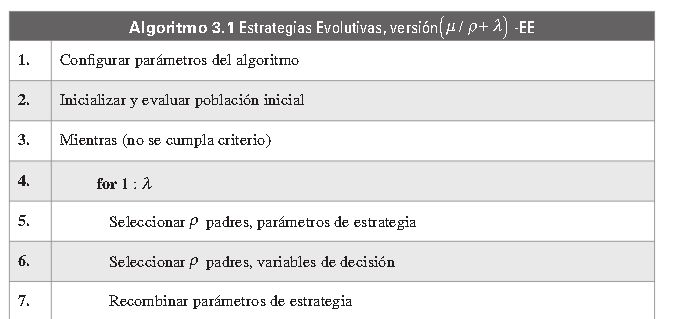
\includegraphics[width=10cm]{imgs/Captura de pantalla 2021-01-19 184554.png}
    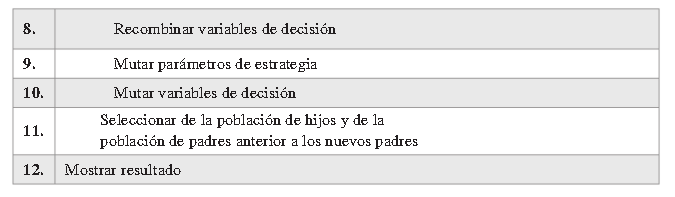
\includegraphics[width=10cm]{imgs/Captura de pantalla 2021-01-19 184634.png}
    \caption{Muestra de un algoritmo evolutivo}
    \label{fig:my_label}
\end{figure}

\footnote{ \cite{Cuevas(2016)} pp 67}


\subsubsection{Evoluci\'on Diferencial}
El algoritmo de Optimizaci\'on Evoluci\'on Diferencial (Differential Evolution, por sus siglas en ingl\'es), es un algoritmo poblacional de b\'usqueda directa y simple, el cual es capaz de optimizar hasta alcanzar el \'optimo global en funciones multimodales, no diferenciales y no lineales. Fue propuesto por \textit{Kenneth Price y Rainer Storn} en $1995$. Desde entonces, el algoritmo DE ha probado sus capacidades en concursos Internacionales de la IEEE en Optimizaci\'on Evolutiva, asi como con grandes aplicaciones en el mundo real.

El DE se basa en perturbar a los miembros de la poblaci\'on generada con diferencias escaladas de distintos miembros de una misma poblaci\'on. Lo hacen caracter\'istico de los dem\'as algoritmos evolutivos dado que esta inspirado en un f\'enomeno biol\'ogico, social, f\'isico o qu\'imico. El algoritmo DE fue dise\~nado para que se cumpliera con (i) capacidad de lidiar con funcio-nes objetivo no diferenciables, no lineales y multimodales, (ii) fácil implementación, (iii) pocos parámetros de ajuste, (iv) propiedades de convergencia consistentes en pruebas consecutivas in-dependientes y (v) capacidad de paralelizarse para lidiar con funciones de alto costo computa-cional. A continuaci\'on se presenta el algoritmo o un diagrama de flujo g\'enerico de las operaciones llevadas acabo por el algoritmo evoluci\'on diferencial.
\begin{figure}[h!]
    \centering
    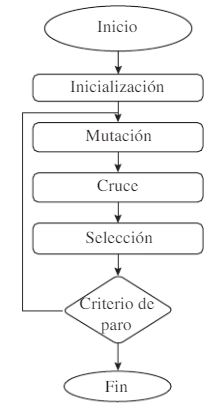
\includegraphics[width=5cm]{imgs/Evolucion diferencial.JPG}
    \caption{Diagrama de flujo de la búsqueda armónica}
    \label{fig:my_label}
\end{figure}
De acuerdo con estudios reportados recientemente, el algoritmo DE ha mostrado un mejor desempe\~no que muchos algoritmos evolutivos en t\'erminos de convergencia, velocidad y robustez sobre distintas funciones de prueba.

\subsubsection{B\'usqueda Arm\'onica}
En este algoritmo se representa a una armonía como en vector $n$-dimensional de números reales.\cite{Coley (1999)}
\begin{itemize}
    \item Un conjunto inicial de vectores de armonía son generados aleatoriamente y almacenados dentro de la memoría de armonías (HM).
    \item Una nueva armonía candidada es calculada a partir de los elementos contenidos en la HM, para esto existe un parámetro conocido como consideración de memoria.
    \item Se actualiza la memoria de armonías, por medio de la comparación de la nueva armonía candidata y el peor de los vectores de armonía. 
\end{itemize}
\begin{figure}[H]
    \centering
    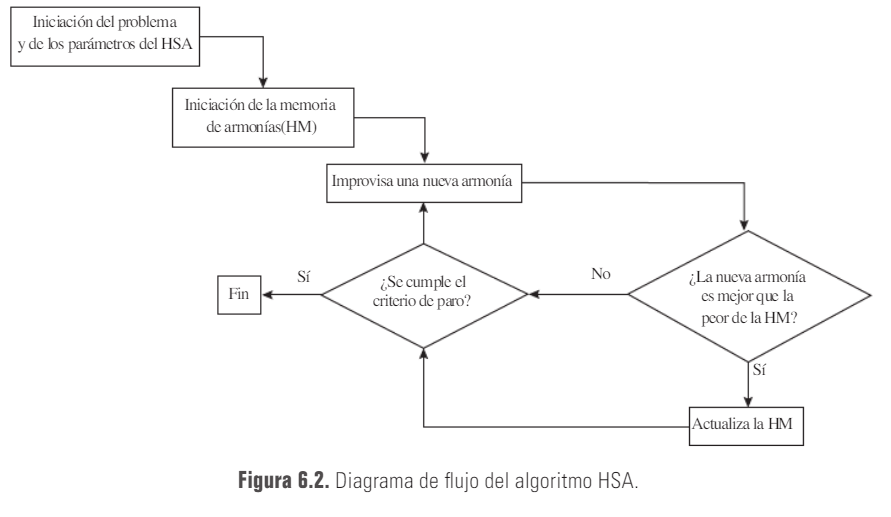
\includegraphics[scale=0.6]{imgs/hsa_diagrama.png}
\end{figure}
Un popularidad del algoritmo HSA se debe a un conjunto de características que lo distinguen del resto de los algoritmos metaheurísticos. Algunas de éstas son: \\ 
1. Para generar nuevas soluciones se consideran todas las soluciones existentes, no sólo dos de ellas como los padres en los algoritmos genéticos. \\ 
2. Se considera de forma independiente cada variable de decisión en un vector de soluciones. \\
3. Los valores de las variables de decisión son continuos, por lo que no se pierde precisión.

\subsubsection{Sistemas Inmunológicos Artificiales}
Para definir lo que es un sistema inmune artificial recurriremos a una de
las definiciones más completa propuesta por Leandro Nunes de Castro y
Jonathan Timmis.\\Los sistemas inmunes artificiales son sistemas adaptativos, inspirados por la teoría inmunológica, funciones, principios y modelos inmunológicos observados, los cuales son aplicados a la
solución de problemas.\\
Aunque la cantidad de modelos y aplicaciones del sistema inmune va en
ascenso, no existe un esquema general de cuáles son los elementos esenciales
que un sistema inmune artificial debe poseer. \\
Nunes De Castro y Timmis sugieren en su libro utilizar un esquema
general de sistemas computacionales con inspiración biológica, tal como los
algoritmos evolutivos o las redes neuronales. Este esquema consta de tres
partes principales que deben denirse, y que a continuación se muestran:

\begin{itemize}
  \item  Representación de los componentes del sistema.
  \item Un conjunto de mecanismos para evaluar las interacciones de los individuos con el ambiente y entre ellos.
  \item Un proceso de adaptación que gobierne las dinámicas del sistema, es
decir, el algoritmo en sí.
\end{itemize}

 Representación de los componentes del sistema.\\
 Un conjunto de mecanismos para evaluar las interacciones de los individuos con el ambiente y entre ellos.\\
 Un proceso de adaptación que gobierne las dinámicas del sistema, es
decir, el algoritmo en sí.\\

A diferencia de otras técnicas bio-inspiradas (por ejemplo los algoritmos
genéticos), el sistema inmune artificial no tiene un algoritmo general único.\cite{Cuevas(2016)}

\subsubsection{Optimizaci\'on basada en electromagnetismo}
El algoritmo EMO es un método basado en población propuesto por Birbil y Fang  para resolver modelos de optimización continuos usando variables acotadas. Es decir,  problemas de optimización.
El algoritmo EMO replica el problema de las cargas, donde cada carga representa una solución a un campo dado, lo cual representa que cada cantidad de carga es una parte de la solución y refleja su cálidad. Este algoritmo, permite encontrar solución a problemas de minimización del tipo $f(X) X \epsilon [l,u]$ a través de los siguientes cuatro pasos.

\begin{itemize}
    \item Inicialización: un conjunto de m partículas son tomadas aleatoriamente considerando un espacio $R$ definido por el límite superior u y el límite inferior l
    \item Búsqueda local: se realiza la búsqueda de un valor mínimo en la vecindad de un punto $X_p$, donde $ p \epsilon [m1,m2]$ y m es el número total de individuos de la población.
    \item Cálculo del vector de fuerza total: con base en el valor de la función objetivo se calculan las cargas y fuerzas para cada elemento de población de partículas.
    \itemMovimiento: cada partícula de población es desplazada de acuerdo a la fuerza total calculada con base en el valor de la función objetivo.\footnote{El ejemplo fue obtenido de \cite{Cuevas(2016)}}
\end{itemize}
\begin{verbatim}
%Inicializacion, Algoritmo EMO Standar
%Prueba con función de Rosenbrock
function [x.fx] = inicializa (m,n,u,l)
%Se genera las partículas de forma aleatoria en el espacio de búsqueda
for i = 1:n
%Se obtiene el número aleatorio
lambda= rand(l,m);
	x(i,:) = l(i) + lambda * (u(i) -l(i));
end
%Se evalúa cada partícula en la función objetivo (Rosenbrock)
for j =1:m
	fx(j) = rosen(x(:,j));
end             
\end{verbatim}

El código anterior es una implementación del algoritmo EMO para la función de Rosenbrock.
\subsubsection{Colonia Artificial en Abejas, Hormigas}
El problema de optimización de colonia, es una tecnica probabilística para resolver problemas computacionales que pueden ser reducidos a encontrar un camino bueno en una gráfica. \\ 

La forma más fácil de entender como el algoritmo de optimización por colonia de hormigas funciona, es a través de un ejemplo. Consideremos el problema del agente viajero, consiste en, dado un conjunto de ciudades y la distancia entre estas, encontrar la ruta más corta que visite a todas y regrese al lugar de partida. \\

Las hormigas construyen la solución de la siguiente manera. Cada hormiga selecciona una ciudad aleatoria. Después, en cada paso se mueve a un nuevo vértice queno haya sido visitado de forma probabilística, esta decisión esta basada en información como la feromona. Cada vez que una hormiga finaliza su recorrido, la feromona de cada arista es actualizado de acuerdo a la calidad de la solución resultante.

\newpage 
\section{Estudio y evaluación de un algoritmo evolutivo, de manera que se pueda implementar de manera concurrente.}
\subsection{Estudio y evaluación}
El algoritmo genético como ya mencionamos en la sección anterior, es un algoritmo que restringe una búsqueda con los siguientes pasos.
\begin{itemize}
    \item Generar población inicial.
    \item Seleccionar de esta población individuos más capacitados.
    \item Reproducir y mutar estos individuos.
    \item Obtiene una nueva generación de individuos mejor adaptados
    
\end{itemize}
El proceso se repite hasta llegar a una solución aceptable.
El algoritmo genético podemos notar que se basa de un sistema de selección natural, en el cual tras cada iteración solo los individuos más aptos sobreviven, y que por tanto serán base para las generaciones posteriores.
Esta capacidad les permite resolver muchos problemas que no son de un campo en específico. Solo debemos definir un problema y una función de evaluación de los individuos para poder resolver cualquier tipo de problema. Al tratarse de una técnica heurística el tiempo de ejecución puede volverse un obstáculo si el espacio de búsqueda de soluciones es muy amplio, además de que si el factor de mutación no es elegido con cuidado, podríamos hacer un algoritmo que no convergiese a el óptimo buscado. Por eso es necesario garantizar la diversidad de los individuos al realizar la técnica, y también es esta complicación por la cual es natural aplicar paralelización, precisamente en la subsección siguiente discutiremos esto con más profundidad, para dar la justificación a la elección de un algoritmo genético.\cite{Coley (1999)}

\begin{figure}[htb]
\begin{center}
\leavevmode

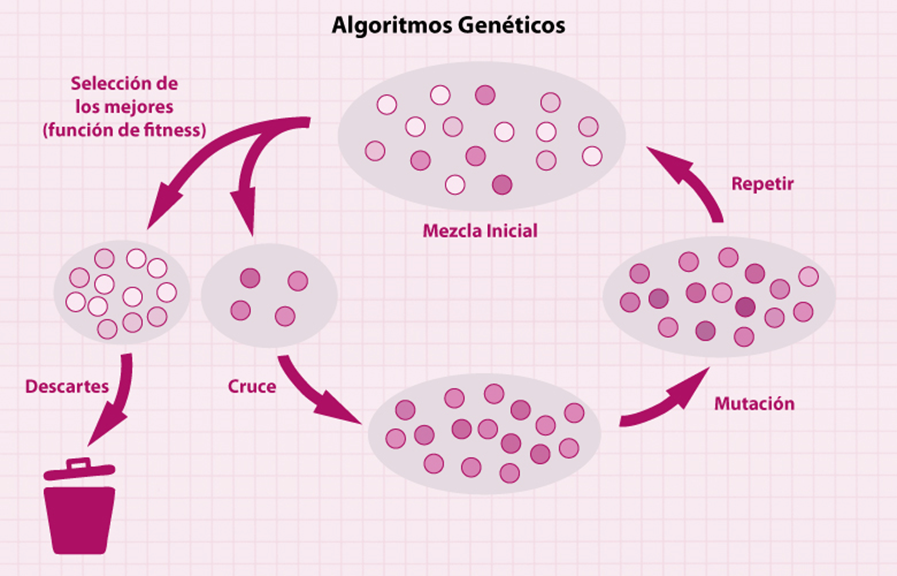
\includegraphics[width=0.8\textwidth]{ALGORITMOGENETICO2.png}   
\end{center}
\caption{Esquema gráfico de ciclo del algoritmo genético.}
\label{fig:awesome_image}
\end{figure}

\subsection{Justificación}
Decidimos elegir el algoritmo genético dado que la labor de selección de los individuos, es una tarea que se puede paralelizar y que además no afecta la solución final del algoritmo. La selección debe ser realizada de manera global si queremos que el algoritmo produzca el mismo resultado que la secuencial original. Para paralelizar nuestro algoritmo, se puede optar por generar grupos pequeños de poblaciones que se comuniquen entre ellas en lugar de generar una población muy grande, de acuerdo a la bibliografía más apremia, realizar una paralelización en este punto puede ser incluso más favorable que el algoritmo secuencial.de hecho este proceso de paralelización se conoce como generar nichos.  \footnote{Esto lo obtuvimos del artículo \cite{S. Poddar, 2020} }
\begin{figure}[h!]
    \centering
    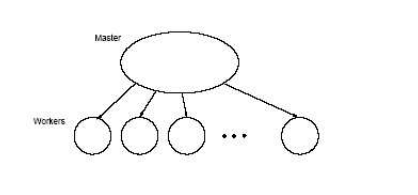
\includegraphics[width=9cm]{imgs/AGP.png}
    \caption{Diagrama proceso de paralelizacion tipo maestro-trabajador}
    \label{fig:my_label}
\end{figure} 




Esta es una representación esquemática de un algoritmo genético paralelizado, con la aplicación del proceso paralelo en la evaluación de los individuos, ya que suele ser también la que toma más tiempo. 

    El intercambio de información entre los nodos 
realiza los siguientes pasos
\begin{itemize}
    \item Nodo maestro envia subconjunto de individuos a cada nodo. 
    \item Cada nodo retorna el valor de evaluación al nodo maestro.
    
\end{itemize}
De forma tradicional, el nodo maestro espera a recibir los valores de adecuación de todos los individuos para hacer la siguiente generación, pero también podemos hacer que los nodos más lentos no se comuniquen con el nodo maestro, aunque aquí perderíamos información del comportamiento original.

\begin{figure}[h!]
    \centering
    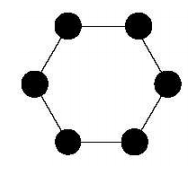
\includegraphics[width=5cm]{imgs/arqui2.png}
    \caption{Diagrama de paralelización de poblaciones distribuidas.}
    \label{fig:my_label}
\end{figure}




Una segunda forma de generar paralelización, es generar una arquitectura de muchas poblaciones, este es el caso en donde cada sub población es repartida hacía un diferente procesador y es evaluada por separado. Se encontró que en está arquitectura, las poblaciones por separado convergen más rápido hacía valores óptimos, aunque en contraste, estos valores no son tan buenos como los del proceso secuencial.\cite{parallelgenetic2011}

\section{Problema de aplicación elegido en el punto anterior}

En nuestro trabajo deseamos encontrar un coloración de una gráfica aleatoria dada \footnote{Se dice que hay una coloración de la gráfica si para cualesquiera dos vértices adyacentes estos dos estan coloreados de diferente color} de la gráfica
El problema de colorear una gr\'afica es un problema bastante conocido de tipo \textit{NP-Completo}.El coloreado de una gr\'afica incluye tanto a los v\'ertices como a las aristas. Sin embargo, el t\'ermino de coloreo de una gr\'afica se refiere a colorear los v\'ertices en vez de al coloreado de aristas.\\ 

Dados un n\'umero $n$ de v\'ertices, que forman una gr\'afica conexa, el objetivo es colorear cada v\'ertice de manera que dos v\'ertices vecinos (i.e. adyacentes) sean coloreados de manera diferente. Claramente esta tarea se puede realizar si el número de colores que usamos es mayor al número de vértices, por esta razón definimos el número cromático $\chi$ de una gráfica como el número de colores más pequeños que se necesita para tener una coloración correcta.\cite{Prugel-Bennett, A. 2003. Genetic algorithm for graph coloring} \\ 

Una herramienta que es útil en este contexto es el teorema de los cuatro colores, el cual nos dice que dada una gráfica plana \footnote{Se dice que una gráfica es plana, si es posible dibujarla en el plano de manera que no haya dos aristas que se crucen entre ellos,el teorema de Euler, que nos dice que dada una gráfica, está es plana, si dadas sus caras, vértices y aristas, el número de vértices menos el número de aristas mas el numero de caras es exactamente igual a dos} esta se puede colorear con únicamente 4 colores\cite{Prugel-Bennett, A. 2003. Genetic algorithm for graph coloring}
Nuestro problema es un poco más general, pues para cualquier gráfica no necesariamente plana, necesitamos encontrar una coloración, para la cual podemos requerir de $1$ hasta $n$ colores.
\begin{figure}[h!]
    \centering
    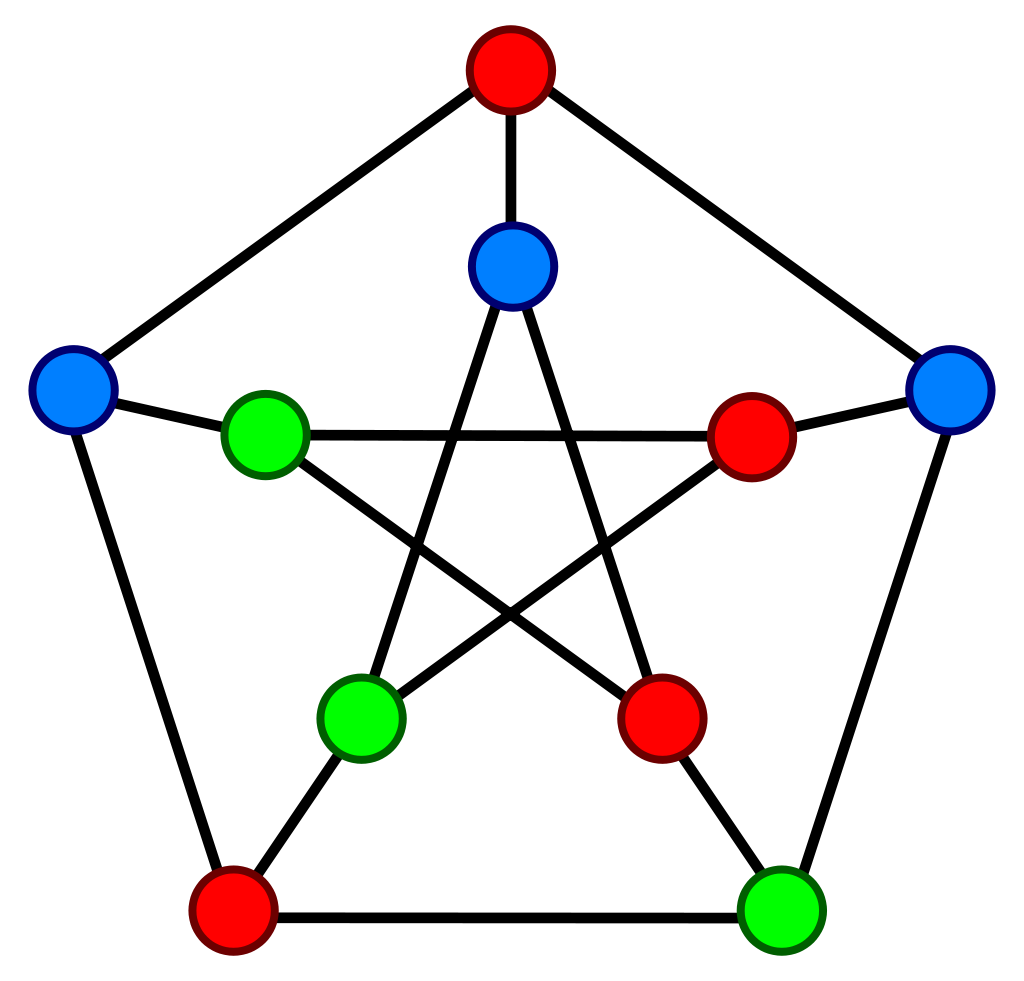
\includegraphics[width=5cm]{imgs/graph_3color.png}
    \caption{Gráfica coloreada con 3 colores.}
    \label{fig:my_label}
\end{figure}

\subsection{Contribución del algoritmo evolutivo para resolver el problema}
Observe que si $k$ es el número de colores necesarios para hacer una coloración de nuestra gráfica, podemos encontrar dicha coloración a partir de un algoritmo genético.
Un algoritmo genético es ideal para resolver este problema, pues podemos pensar a la persona más apta como aquella que tiene más aristas coloreados con vértices de diferente color, lo ideal seria que todos los aristas de nuestra gráfica cumplieran dicha condición, así podríamos comenzar con una población inicial, que seria un conjunto de coloraciones aleatorias, e ir seleccionando aquellas que sean más aptas, es decir, aquellas que tienen más aristas coloreados con vértices de distinto color y cruzarlas entre ellas para obtener una nueva población de manera que obtengamos cada vez mejores coloraciones.
%holi

\cite{M. Hindi and V.Yampolskiy, 2011}

Diremos que hemos encontrado una coloración valida cuando el número de aristas que tengan 2 vértices adyacentes coloreados de distinto color, sea igual al número de aristas de nuestra gráfica.

\newpage 
\section{Análisis diseño e implementación de la paralelización del algoritmo.}
\subsection{Diseño}
\subsubsection{Definiciones}
En este caso se tienen las siguientes definiciones:
\begin{itemize}
    \item \textbf{Person}: Una coloración arbitraria de la gráfica, esta se puede ver como una lista que nos indica el color de cada vértice $[1,0,2,1,...,0]$.
    \item \textbf{Fitness}: Número de aristas que conectan a dos vértices de distinto color.
    \item \textbf{Crossover}: Dadas 2 coloraciones (padres) elegimos un número aleatorio entre $0$ y $n$, y creamos una nueva coloración que tenga los primeros $k$ colores iguales a los de la primera y el resto igual a los de la segunda.
    \item\textbf{Mutation}: Dada una coloración, tomar un vértice arbitrario y cambiar su color.
\end{itemize}

\subsubsection{Algoritmo}
En resumen se podría diseñar nuestro algoritmo de la siguiente manera:
\begin{enumerate}
    \item Generar población aleatoria (primer generación). Nuestra población seria un conjunto de coloraciones.
    \item Distribuir a la población en islas, cada isla evolucionará de manera independiente. Para cada isla:
    \item Obtener fitness para cada individuo. Número de aristas que conectan 2 vértices de distinto color.
    \item Seleccionar padres, favoreciendo aquellos que hayan obtenido un mayor fitness.
    \item Hacer crossover y mutaciones para obtener nueva generación.
    \item Repetir paso 2, según el número de generaciones que deseemos.
    \item Obtener el individuo con mayor fitness para cada isla, el mejor de estos será la coloración que usaremos (the best of the best).
\end{enumerate}
\subsubsection{Parámetros}
Del algoritmo se tienen los siguientes parámetros:
\begin{itemize}
    \item \textbf{G}: Gráfica que se desea colorear.
    \item \textbf{population\_size}: Número de personas en la población.
    \item \textbf{n\_islands}: Número de islas en las que se distribuirá la población.
    \item \textbf{n\_generations}: Número de generaciones que se usarán para evolucionar a la población.
    \item \textbf{percentage\_to\_keep}: Porcentaje de la población con mejor fitness que se copia de a la siguiente generación. 
    \item \textbf{n\_colors}: Número de colores con los que se planea colorear la gráfica.
\end{itemize}

\subsubsection{Como medir performance}
Para evaluar nuestras soluciones, contamos con gráficas previamente estudiadas para las cuales su número cromático $\chi$ es conocido (Figura \ref{table:dimacs_graphs}). Obtenidas del \textit{Center for Discrete Mathematics and Theorical Computer Science} (DIMACS) challenge \cite{Graph colors instance}, el cual es un conjunto comúnmente usado para medir el performance de este tipo de algoritmos .
De esta forma, esperamos que fitness\_percentage, definido como:
\begin{equation*}
    fitness\_percentage = \frac{\#AristasColoreadas}{\#Aristas}
\end{equation*}
sea 1 o muy cercano a 1, pues sabemos que existe una solución, y podemos entonces evaluar el tiempo de ejecución y velocidad de convergencia. 
\begin{figure}[H]
    \centering
    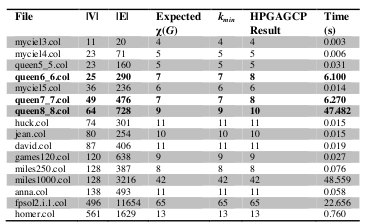
\includegraphics[width=13cm]{imgs/datos.png}
    \caption{Datos de gráficos conocidos estudiados con HPGAGCP}
    \label{table:dimacs_graphs}
\end{figure}
Podemos notar en la Figura 9 \footnote{ Table 1: Results of running the proposed algorithm on 16 .col
files from the DIMACS collection en \cite{M. Hindi and V.Yampolskiy, 2011}} que estas gráficas previamente estudiada, cuentan con diferentes características, van de los 11 vértices a los 561, y van desde 20  a  3216 aristas , esto significa que tenemos una muestra muy amplia de casos de estudio que nos permitirán evaluar y validar nuestro algoritmo. Contamos también con la cantidad de colores necesarios para cada gráfica y el tiempo de ejecución con el algoritmo HPGAGCP. \footnote{El algoritmo HPGAGCP viene descrito en la sección Proposed Approach en \cite{M. Hindi and V.Yampolskiy, 2011}}

%\begin{multicols}[2]
Para la simulación se utilizara python y la libreria networkx junto con matplotlib asi como multiprocessing lo que nos permitirá implementar nuestro algoritmo de manera paralela.
\newpage 
\subsection{Implementación del algoritmo evolutivo de manera concurrente}
El algoritmo principal quedaría de la siguiente manera: 
\begin{figure}[H]
    \centering
    \subfloat{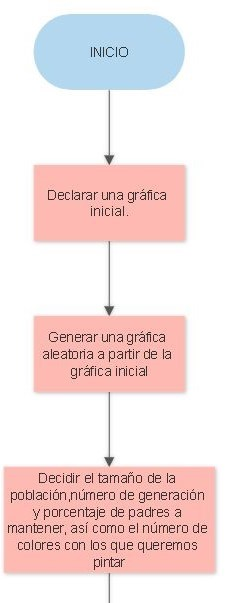
\includegraphics[width=5cm]{principal1 (2).jpg}}
    \quad
    \subfloat{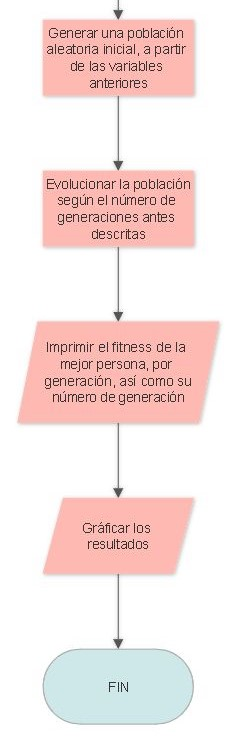
\includegraphics[width=5cm]{principal2.jpg}}
    \caption{Algoritmo principal sin concurrencia}
\end{figure}
\newpage

Observe que el tiempo de ejecución de evolucionar nuestra población depende directamente de el tamaño de nuestra población pues debemos generar tantos hijos como población tengamos, tener una población grande nos trae beneficios como mejorar nuestros individuos más rápido, sin embargo esto trae consigo la desventaja de hacer el programa más lento pues necesitamos calcular el fitness de cada gráfica en nuestra población así como generar más hijos, observe que podemos solucionar este problema implementando un algoritmo concurrente que evolucione cierta parte de nuestra población es decir crear nichos, un problema que tuvimos al implementar este programa es que en principio, podríamos pensar que es mejor crear un proceso tal que para cada individuo en nuestra población calcule su fitness por separado y de hay evolucionar nuestra población, sin embargo esto en vez de mejorar el programa lo hacia más lento, pues el número de procesos que debíamos de crear eran tantos como el número de individuos de nuestra población por el número de generaciones que queríamos generar.
para la solucionar nuestro problema optamos por generar islas, de manera que cada isla tuviera cierto porcentaje de nuestra población y cada proceso se encargara de evolucionarlas por separado para finalmente compararlas entre ellas y encontrar la mejor coloración posibles, de esta manera la implementación de la imagen anterior se mejoro de la siguiente manera:

\begin{figure}[H]
    \centering
    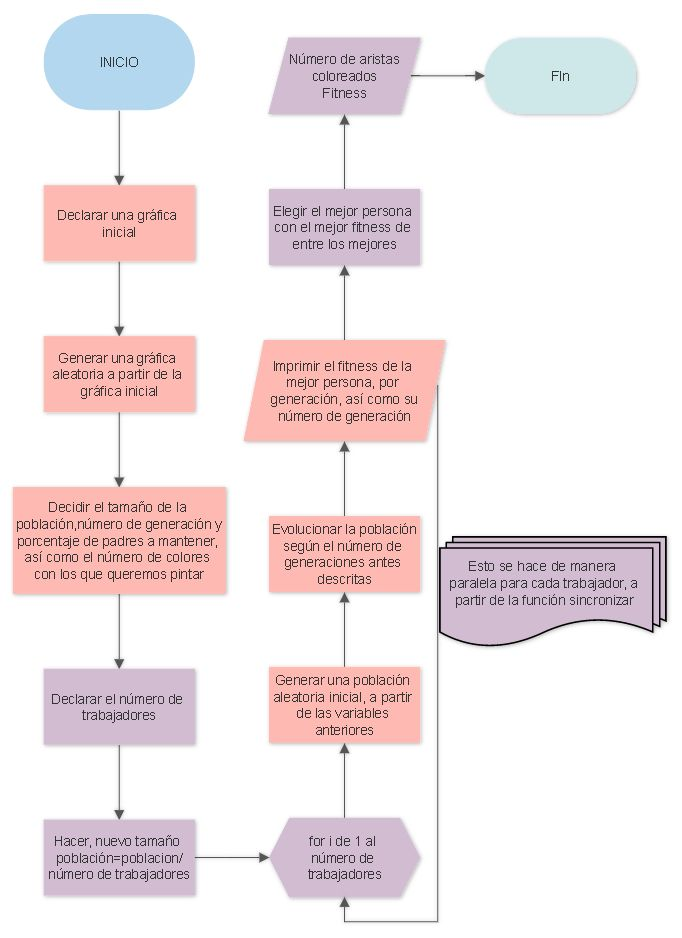
\includegraphics[width=12cm]{main_paral.jpg}
    \caption{Algoritmo principal con una implementación concurrente}
    \label{fig:my_label}
\end{figure}
Como se puede observar para la implementación de manera concurrente, agregamos una nueva función que es la función sincronizar, esta se encargaría de hacer lo siguiente:
\begin{figure}[H]
    \centering
    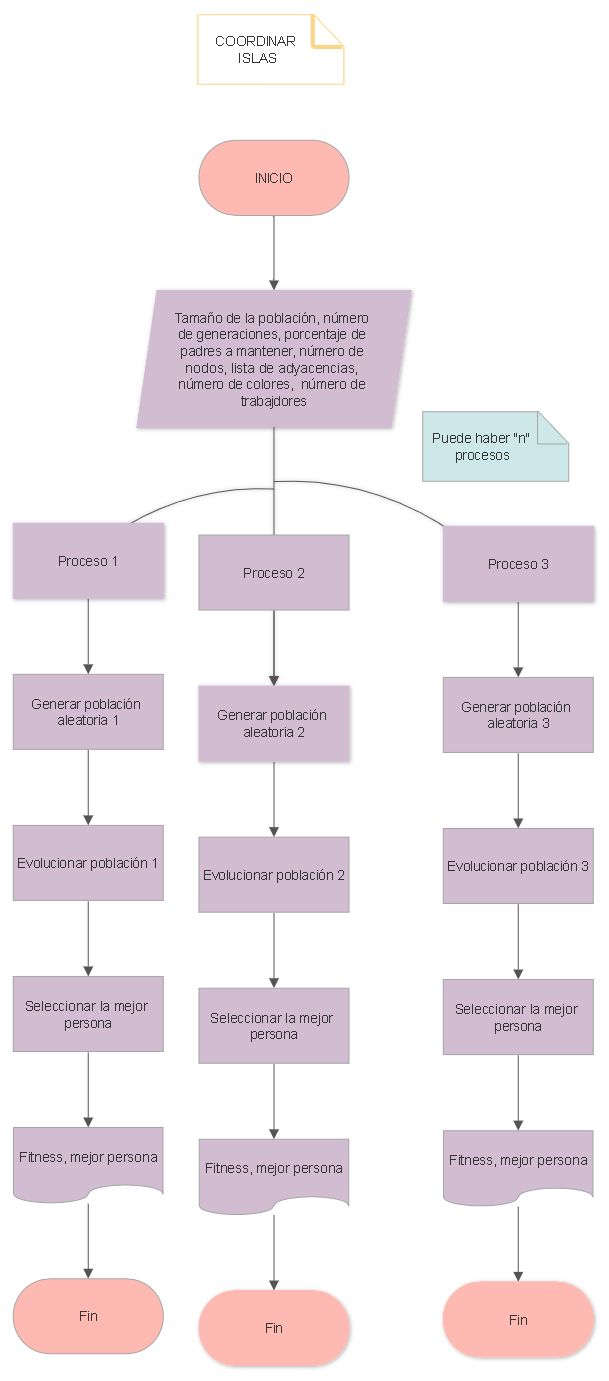
\includegraphics[width=9cm]{islas.jpg}
    \caption{Algoritmo principal con una implementación concurrente}
    \label{fig:my_label}
\end{figure}
Es decir ahora lo que hacemos es evolucionar a cierta parte de la población de manera separada para luego elegir el fitness del mejor individuo.
%\newpage
Podemos también obtener información más detallada de lo que hacen las funciones, generar población aleatoria y evolucionar población en los siguientes diagramas.
%Estrcutura de solucion de generar la poblacion
\begin{figure}[H]
    \centering
    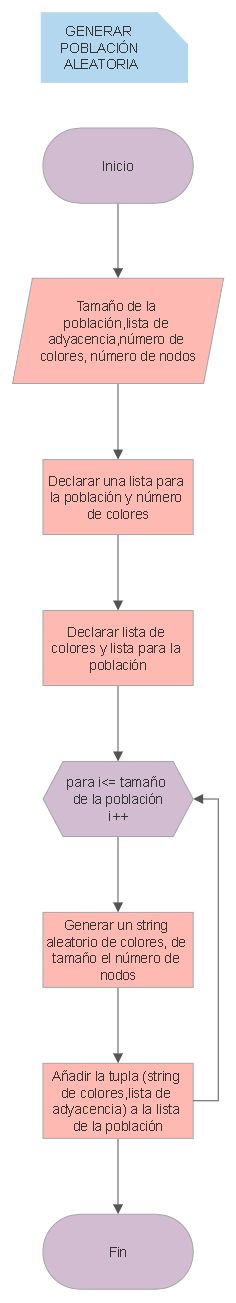
\includegraphics[width=4cm]{flujo_poblacion.jpg}
    \caption{Algoritmo para generar una población aleatoria}
    \label{fig:my_label}
\end{figure}
\newpage
%Estrcutura de evolución de la poblacion
\begin{figure}[H]
    \centering
    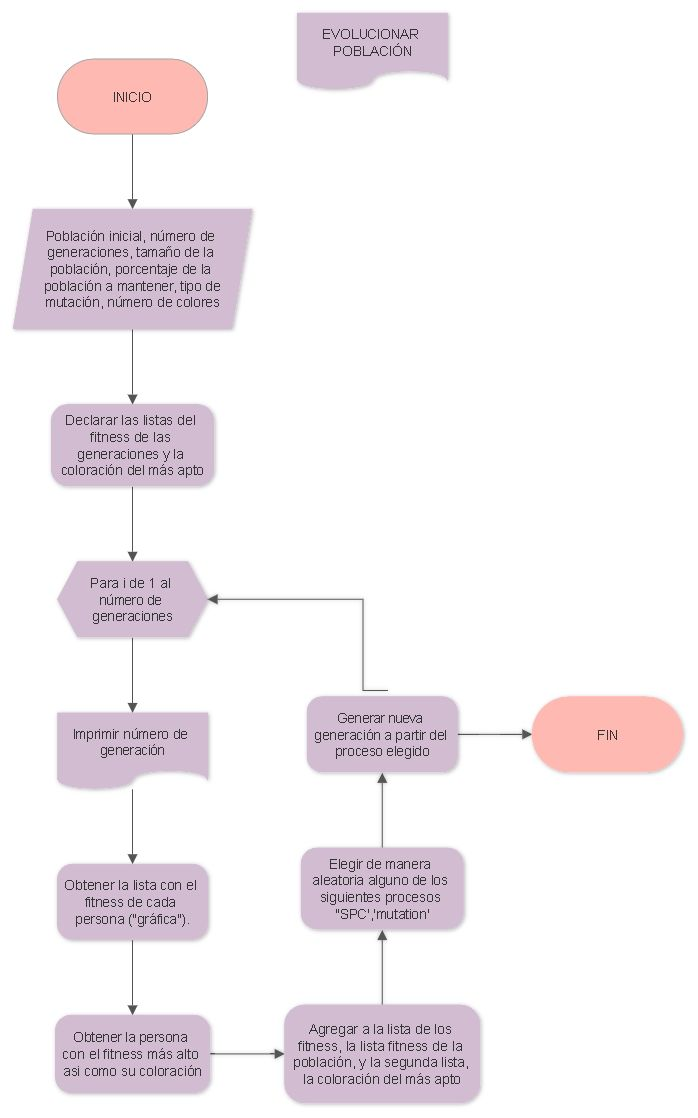
\includegraphics[width=12cm]{flujo_evol.jpg}
    \caption{Algoritmo para evolucionar población}
    \label{fig:my_label}
\end{figure}
\newpage

\section{Documentación del Programa}
En esta sección documentamos las funciones principales de nuestro programa, para no pegar todo el código solo pondremos que parámetros reciben así como lo que nos regresa cada función, nota los diagramas que describen el funcionamiento del programa se encuentran en la sección anterior. La implementación se realizo usando como base al código libre hecho por Jan Krepl \cite{Graph Colouring Repository}.
\small{ 
\begin{minted}{python}
class Coloration:
    def __init__(self, colors, adj):
        """
        Creacion de un objeto Coloration
        :param colors: 
        :type colors: string - contiene la coloración de la gráfica, si tenemos 3 colores puede ser 'rgggbbrg...'
        :param adj: lista de adyacencia de la grafica 
        :type adj: lista de listas 
        :return: objecto Coloration
        :rtype: Coloration
        """
    def get_fitness(self, colors, adj):
        """
        Obtiene cuantas aristas que conecten a dos vértices de distinto color genera Coloration.
        :param colors:
        :type colors: string - contiene la coloración de la gráfica, si tenemos 3 colores puede ser 'rgggbbrg...'
        :param adj: lista de adyacencia de la grafica 
        :type adj: lista de listas
        :return: fitness de Coloration
        :rtype: int  
        """

def parent_selection(input_population, number_of_pairs, method='FPS'):
    """
    Forma pares de padres, favoreciendo aquellos que tengan un mejor fitnesss
    :param input_population: poblacion de la que se desea obtener pares de padres
    :type input_population: lista de coloraciones
    :param number_of_pairs: numero de pares de padres deseados
    :type number_of_pairs: int
    :param method: metodo de seleccion
    :type method: str
    :return: lista de tuplas de pares de padres 
    :rtype: lista de tuplas de Coloration
    """

def genetic_operator(pair_of_parents, method='SPC', n_colors=3):
    """
    Dados dos padres, regresa dos hijos resultantes de la cruza de estos
    :param pair_of_parents: par de padres 
    :type pair_of_parents: lista que contenga dos padres
    :param method: metodo de cruza 
    :type method: str
    :param n_colors: colores con los que se desea colorear la gráfica
    :type n_colors: int 
    :return: par de hijos
    :rtype: par de Coloration
    """

def population_update(input_population, percentage_to_keep=0.1, genetic_op='mutation', n_colors=3):
    """
    Evoluciona la población input_population en una generación
    :param input_population: poblacion de la que se desea obtener pares de padres
    :type input_population: lista de Coloration
    :param percentage_to_keep: porcentaje de individuos que se preservan para la siguiente generación
    :type percentage_to_keep: int
    :param genetic_op: metodo de cruza 
    :type genetic_op: str
    :param n_colors: colores con los que se desea colorear la gráfica
    :type n_colors: int 
    :return: población evolucionada en una generación
    :rtype: lista de Coloration 
    """

def generate_random_initial_population(population_size, n_nodes, adj, n_colors):
    """
    Genera una nueva población de manera aleatoria
    :param population_size: tamaño de la población
    :type population_size: int
    :param n_nodes: número de nodos
    :type n_nodes: int
    :param adj: lista de adyacencia de la gráfica que se desea colorear
    :type adj: lista de listas
    :param n_colors: colores con los que se desea colorear la gráfica
    :type n_colors: int 
    :return: población aleatoria 
    :rtype: lista de objetos Coloration
    """
    
def find_fittest(input_population):
    """
    Encuentra Coloration con mayor fitness de input_population
    :param input_population: poblacion de la que se desea obtener pares de padres
    :type input_population: lista de coloraciones
    :return: Coloration con mayor fitness de input_population
    :rtype: Coloration
    """
    
def evolution(input_population, n_generations, percentage_to_keep, n_colors, n_edges):
    """
    Regresa lista con la persona con mayor fitness para cada generación
    :param input_population: poblacion de la que se desea obtener pares de padres
    :type input_population: lista de Coloration
    :param n_generations: número de generaciones a simular
    :type n_generations: int
    :param percentage_to_keep: porcentaje de individuos que se preservan para la siguiente generación
    :type percentage_to_keep: int
    :param n_colors: colores con los que se desea colorear la gráfica
    :type n_colors: int 
    :param n_edges: número de aristas en la gráfica que se desea colorear 
    :type n_edges: int 
    :returns: Lista con la persona con mayor fitness para cada generación
    :rtype: Coloration
    """
    
def visualize_results(islands_fittest, n_edges):
    """
    Genera visualización de generación vs fitness para cada isla 
    :param islands_fittest: contiene listas del fitness para cada isla para cada generación
    :type islands_fittest: lista de listas 
    :param n_edges: número de aristas en la gráfica que se desea colorear 
    :type n_edges: int 
    """
    
def coordinate(population_size, n_generations, percentage_to_keep, n_nodes, n_edges, n_colors, adj, n_islands):
    """
    Crea los procesos que se ejecutan de forma paralela y encuentra el individuo con mayor fitness
    entre todas las islas 
    :param population_size: tamaño de la población que se desea simular
    :type population_size: int
    :param n_generations: número de generaciones a simular
    :type n_generations: int
    :param percentage_to_keep: porcentaje de individuos que se preservan para la siguiente generación
    :type percentage_to_keep: int
    :param n_nodes:
    :type n_nodes:
    :param n_edges: número de aristas en la gráfica que se desea colorear 
    :type n_edges: int 
    :param n_colors: colores con los que se desea colorear la gráfica
    :type n_colors: int 
    :param adj: lista de adyacencia de la gráfica que se desea colorear
    :type adj: lista de listas
    :param n_islands: número de islas en las que distribuira la población (número de procesos que se crearan)
    :type n_islands: int 
    :return: persona con mayor fitness de entre todas las islas
    :rtype: Coloration
    """
    islands_params = [(population_size//n_islands, n_nodes, adj, n_colors)]*n_islands
    with Pool(n_islands) as p:
        islands = p.starmap(generate_random_initial_population, islands_params)

    new_islands_params = [(island, n_generations, percentage_of_parents_to_keep, n_colors, n_edges) for island in islands]
    with Pool(n_islands) as p:
        islands_fittest = p.starmap(evolution, new_islands_params)

    visualize_results(islands_fittest, n_edges)
    
    best_fit = 0
    for island_fittest in islands_fittest:
        best_fit = max(best_fit, island_fittest[-1])
    
    return best_fit

def get_graph(name):
    """
    Regresa número de nodos, número de airstas, número cromatico y matriz de adyacencia de la gráfica name
    :param name: nombre de la gráfica 
    :type name: str
    :return n_nodes, n_edges, n_colors, adj: 
    """
    
if __name__ == '__main__':
    """
    Función principal, aqui se definen todos los parámetros del modelo como population_size,
    n_generations y n_colors.
    """
    names = ['anna', 'david', 'games120', 'homer', 'huck', 'jean', 'miles1000', 'miles250',
    'myciel3', 'myciel4', 'myciel5', 'queen5_5', 'queen6_6', 'queen7_7', 'queen8_8']
    names.sort()
    for graph_name in names:
        t1 = time.time()
        n_nodes, n_edges, n_colors, adj = get_graph(graph_name)
        population_size = 300
        n_generations = 1000 
        percentage_of_parents_to_keep = 0.3
        n_islands = 6
        print('Graph name: ', graph_name)
        print('Number of nodes: ' + str(n_nodes))
        print('Number of edges: ' + str(n_edges))
        print('Number of colors: ' + str(n_colors))
        fittest = coordinate(population_size, n_generations, percentage_of_parents_to_keep,
                             n_nodes, n_edges, n_colors, adj, n_islands)
        print(f'Fittest: {fittest: .2f}')
        t2 = time.time()
        total_time = t2-t1
        print(f"{total_time: .2f}")
\end{minted}
}
\newpage 
\section{Resultados}
\subsection{Descripción de resultados y convergencia de las soluciones}
A continuación el análisis de convergencia para las gráficas de prueba (Table \ref{table:dimacs_graphs}). Se muestra el número de generaciones vs el fitness (en porcentaje) para cada gráfica, se utilizaron los siguientes parámetros para el modelo: 
\begin{itemize}
    \item population\_size = 700
    \item n\_generaciones = 1000 (máximo)  
    \item n\_islands = 6
    \item percentage\_to\_keep = 30 \% 
\end{itemize}
\begin{multicols}{2}
\begin{figure}[H]
    \centering
    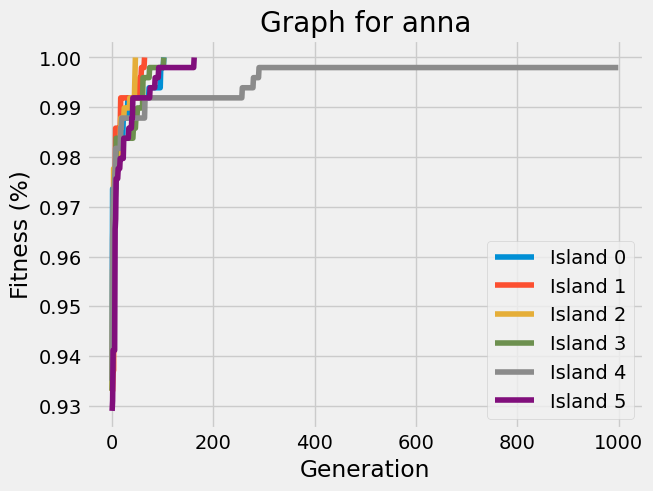
\includegraphics[scale=0.45]{imgs/convergence/anna_evolution.png}
\end{figure}
\begin{figure}[H]
    \centering
    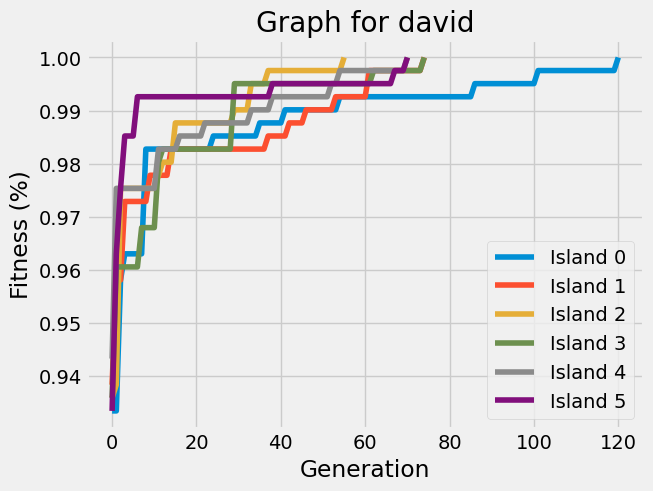
\includegraphics[scale=0.45]{imgs/convergence/david_evolution.png}
\end{figure}
\begin{figure}[H]
    \centering
    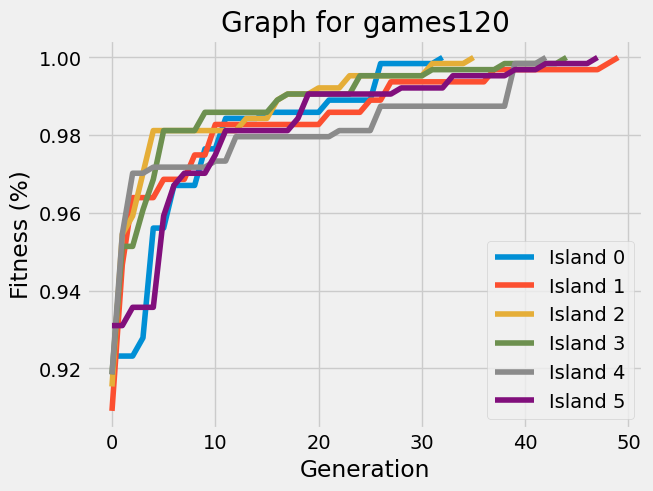
\includegraphics[scale=0.45]{imgs/convergence/games120_evolution.png}
\end{figure}
\begin{figure}[H]
    \centering
    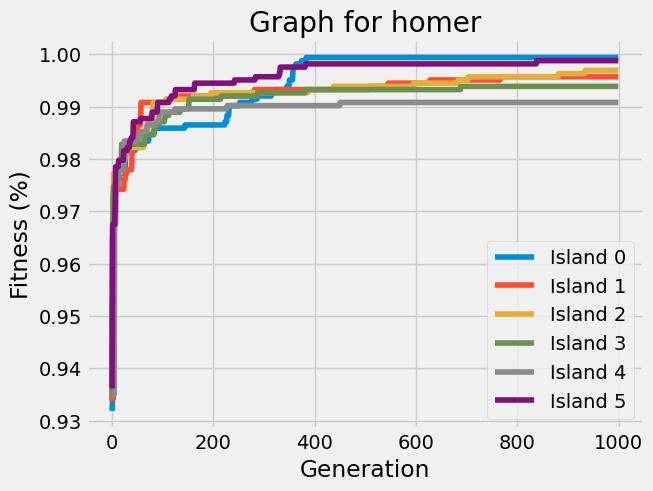
\includegraphics[scale=0.45]{imgs/convergence/homer_evolution.png}
\end{figure}
\begin{figure}[H]
    \centering
    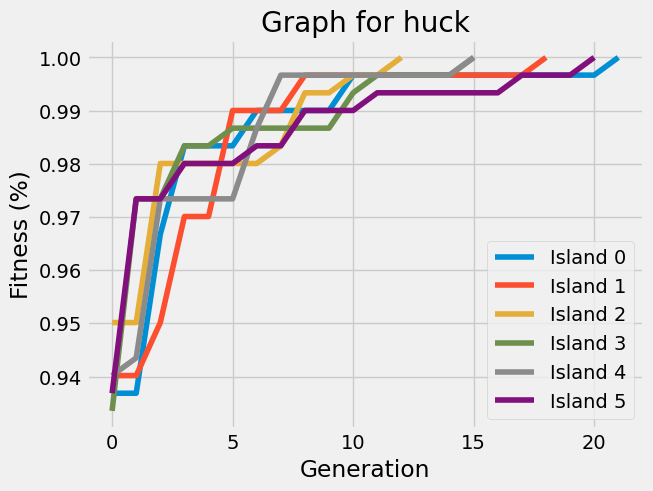
\includegraphics[scale=0.45]{imgs/convergence/huck_evolution.png}
\end{figure}
\begin{figure}[H]
    \centering
    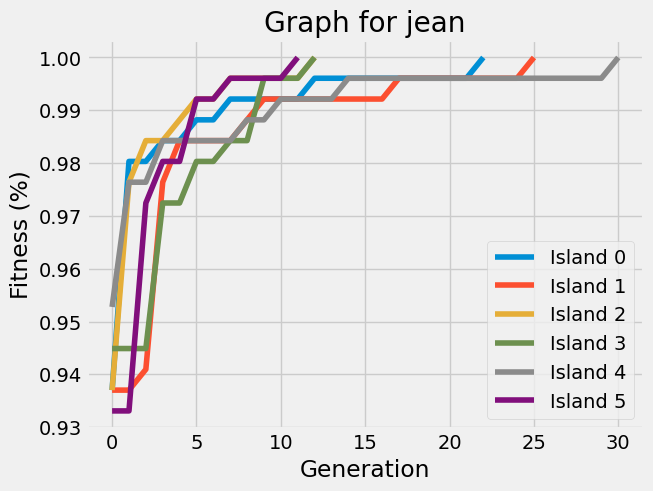
\includegraphics[scale=0.45]{imgs/convergence/jean_evolution.png}
\end{figure}
\begin{figure}[H]
    \centering
    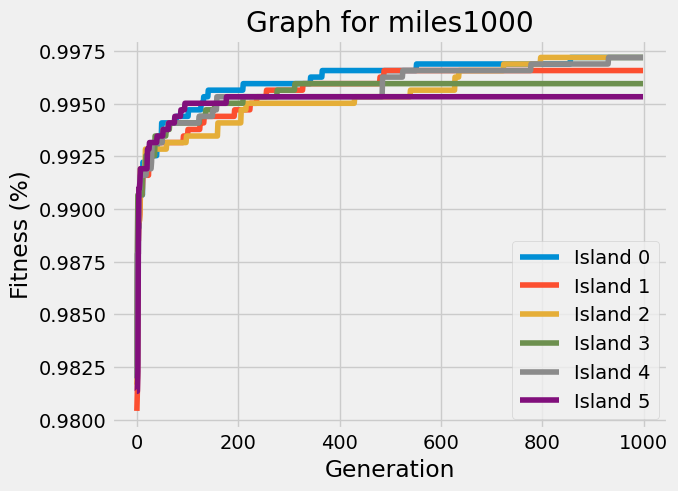
\includegraphics[scale=0.45]{imgs/convergence/miles1000_evolution.png}
\end{figure}
\begin{figure}[H]
    \centering
    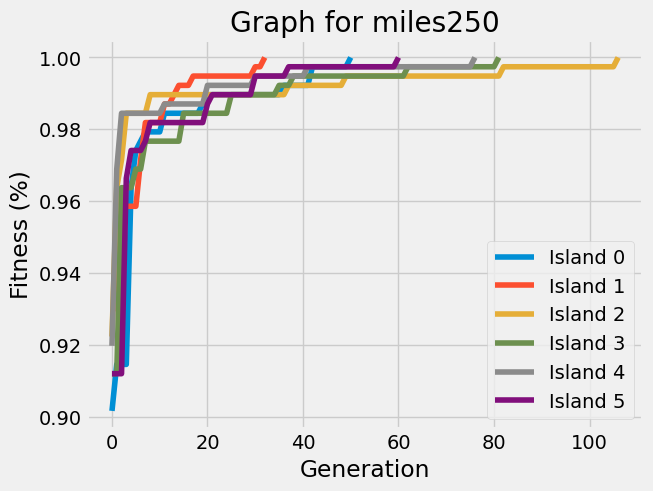
\includegraphics[scale=0.45]{imgs/convergence/miles250_evolution.png}
\end{figure}
\begin{figure}[H]
    \centering
    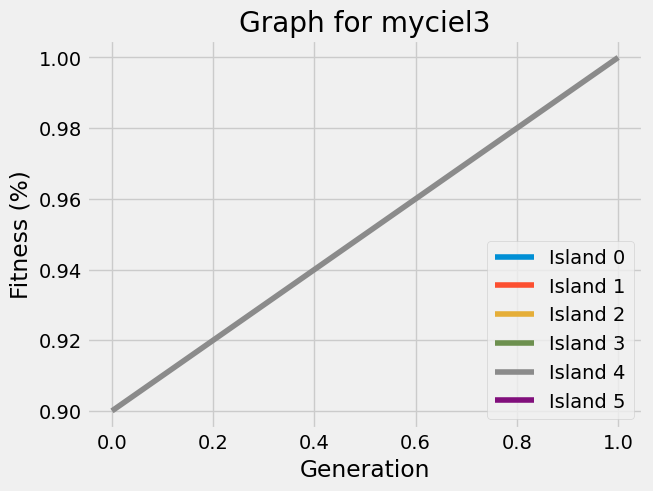
\includegraphics[scale=0.45]{imgs/convergence/myciel3_evolution.png}
\end{figure}
\begin{figure}[H]
    \centering
    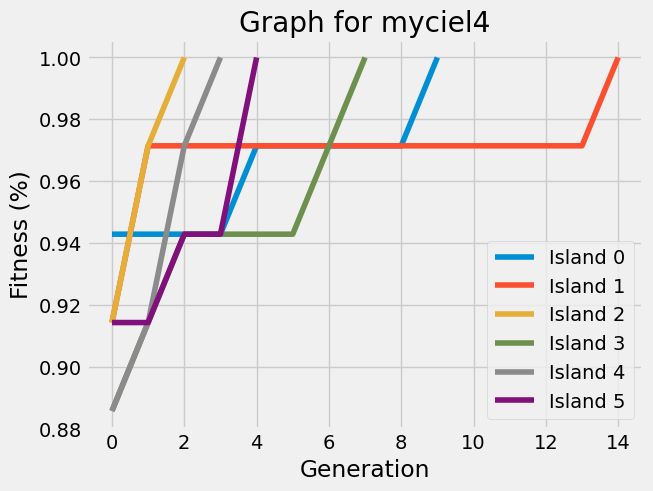
\includegraphics[scale=0.45]{imgs/convergence/myciel4_evolution.png}
\end{figure}
\begin{figure}[H]
    \centering
    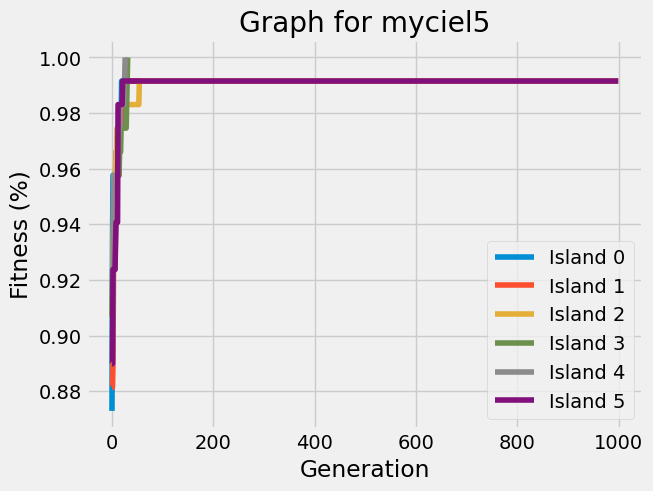
\includegraphics[scale=0.45]{imgs/convergence/myciel5_evolution.png}
\end{figure}
\begin{figure}[H]
    \centering
    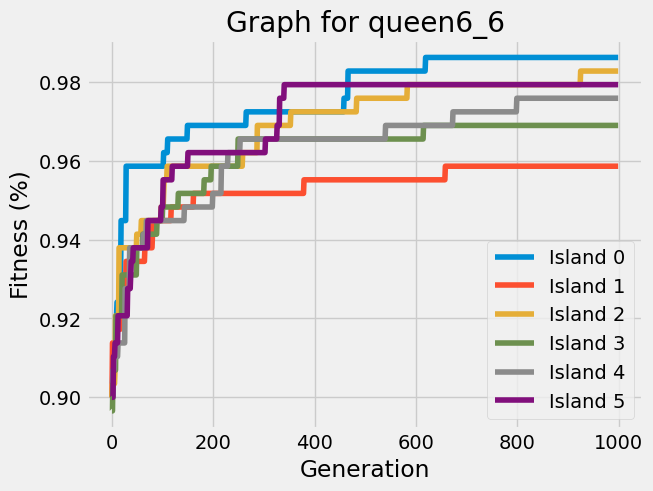
\includegraphics[scale=0.45]{imgs/convergence/queen6_6_evolution.png}
\end{figure}
\begin{figure}[H]
    \centering
    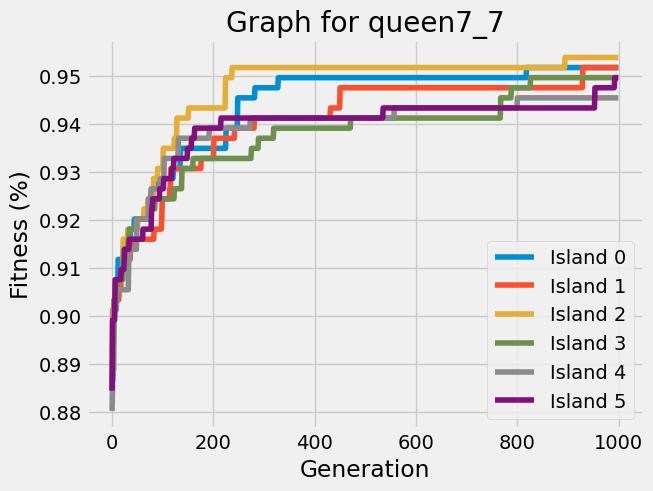
\includegraphics[scale=0.45]{imgs/convergence/queen7_7_evolution.png}
\end{figure}
\begin{figure}[H]
    \centering
    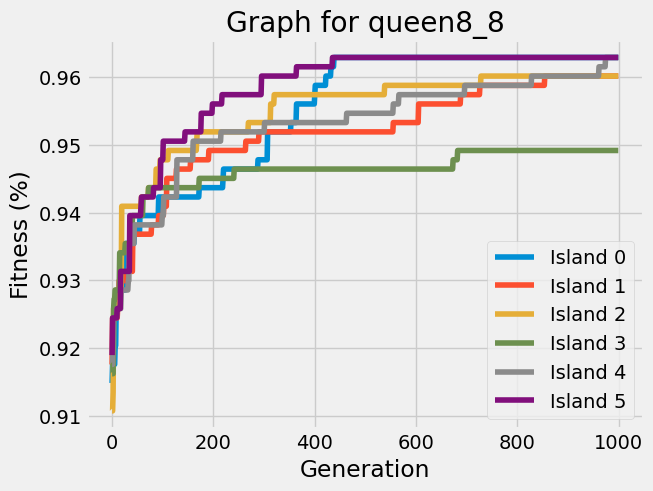
\includegraphics[scale=0.45]{imgs/convergence/queen8_8_evolution.png}
\end{figure}
\end{multicols}
\subsection{Comparación para cada tipo de gráfica.}

La siguiente tabla nos muestra, que porcentaje de aristas fueron coloreadas para las gráficas de prueba (Tabla \ref{table:dimacs_graphs}). Se utilizaron los siguientes parámetros para el modelo:
\begin{itemize}
    \item n\_generations = 4000 
    \item population\_size = 750
    \item n\_islands = 15
    \item percentage\_to\_keep = 30 \%
\end{itemize}
\begin{table}[H]
\centering
\begin{tabular}{|l|l|l|l|l|l|l|}
\hline
Gráfica      & $|V|$  & $|E|$  & #colores   & $|E|$ coloreadas  & Porcentaje    \\ \hline
myciel3     & 11     & 10     &  4         &   10                & 100               \\ \hline
myciel4    &  23    &  35    &5           &   35                & 100           \\ \hline
myciel5  & 36  & 118 & 6                   &  118                 &    100         \\ \hline
queen5\_5  & 23     & 160    &  5         & 160               & 100  \\ \hline
queen6\_6 & 25 & 290 &  7                 & 288               & 99.31  \\ \hline
queen7\_7 &49  & 476  & 7                  &  461              & 96.8       \\ \hline
huck & 74 & 301 & 11                       &   301                &    100         \\ \hline
jean& 80 & 254 & 10                        &254                   &100             \\ \hline
david& 87 & 406 & 11                      & 406               &  100 \\ \hline
games120 &120  &638  & 9                  &  638                 &100        \\ \hline
miles250& 128 & 387 & 8                   &  387                 & 100            \\ \hline
miles1000 &  128 & 3216 & 42              & 3212              &  99.8 \\ \hline
anna& 138 & 493 & 11                       &  493                 &  100           \\ \hline
homer & 561 & 1629 & 13                    &1628                   &100             \\ \hline
\end{tabular}
\end{table}
\footnote{$|V| $Representa los vértices y $|E|$ representa las aristas.}
\subsection{Tiempos de ejecución.}
 Realizamos las ejecuciones correspondientes a cada gráfica con el algoritmo concurrente y su versión secuencial, y comparamos los tiempos de ejecución para hacer una verificación empírica de la eficiencia de nuestra programa.
Para las gráficas conocidas, obtuvimos los siguientes tiempos de ejecución en segundos para ambas versiones del algoritmo la implementación concurrente y la secuencial.

\begin{table}[H]
\centering
\begin{tabular}{|l|l|l|l|l|l|l|}
\hline
Gráfica      & $|V|$& $|E|$&#colores&T Paralelo  & T Secuencial \\ \hline
myciel3   & 11  & 10  & 4 &  13.04  & 61.80 \\ \hline
myciel4   & 23  & 71  & 5 &  20.72  & 86.81 \\ \hline
myciel5   & 36  & 236 & 6 &  38.43  & 219.74 \\ \hline
queen5\_5 & 23  & 160 & 5 &  103.66 & 708.95  \\ \hline
queen6\_6 & 25  & 290 & 7 &  140.51 & 1182.72 \\ \hline
queen7\_7 & 49  & 476 & 7 &  277.09 & 1949.53 \\ \hline
huck      & 74  & 301 & 1 & 53.63   & 396.7 \\ \hline
jean      & 80  & 254 & 10&     50.17   &   352.58 \\ \hline
 david    & 87  & 406 & 11& 53.59   &  377.58 \\ \hline
 games120 &120  & 638 & 9 & 113.55    &    729.09 \\ \hline
 miles250 & 128 & 387 & 8 & 66.13    & 384.33 \\ \hline
 miles1000& 128 & 3216& 42& 444.3   &  3321.67 \\ \hline
anna      & 138 & 493 & 11&  68.15       &  479.34        \\ \hline
homer     & 561 &1629 & 13&    361.60     &   2745.17       \\ \hline

\end{tabular}
\end{table}

\subsection{Análisis de convergencia, tiempos de ejecución y soluciones.}
\subsubsection{Convergencia}
De las gráficas para las cuales implementamos nuestro programa se pueden realizar las siguientes observaciones:
\begin{itemize}
    \item La mayoría de las gráficas con las que implementamos nuestro programa lograron llegar a una coloración óptima o casi óptima.
    \item La mejor solución de la población inicial (aleatoria) suele tener un buen fitness (por arriba del 90 \% en la mayoría de los casos)
    \item La convergencia puede llegar a depender fuertemente de las población inicial (en nuestro caso es aleatoria) como se muestra en $queen8\_8$, donde la isla 3 quedo por debajo de todas las demás, mientras que la isla 5 convergió mucho más rápido que las demás.
    \item Por el punto anteriormente mencionado, el utilizar un mayor número de islas nos asegurara una convergencia más rápida.
\end{itemize}
\subsubsection{Tiempos de Ejecución}
Se muestra una gráfica que compara los tiempos de ejecución del algoritmo secuencial contra el concurrente, algoritmo concurrente en naranja y paralelo en azul
\begin{center}
\begin{figure}[H]
    \centering
    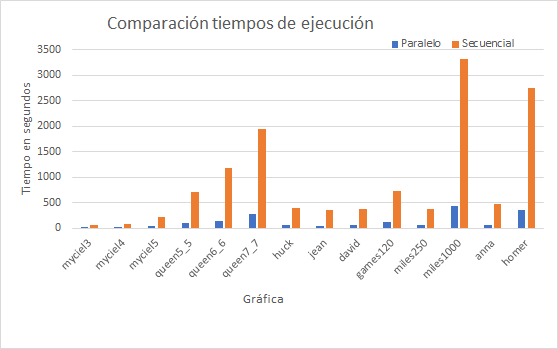
\includegraphics[width=15cm]{ejec1.png}
    \caption{Comparación de tiempos de ejecución de algoritmo concurrente y secuencial.}
    \label{fig:my_label}
\end{figure}
\end{center} 
Observe que el tiempo de ejecución es de 3 a 6 veces mejor dependiendo de la gráfica que estemos coloreando.\\
Por otra parte podemos hacer un análisis de  los tiempos de ejecuci\'on al variar el n\'umero de procesos con respecto a las gr\'aficas \textit{myciel3, myciel4, myciel5}, como se puede ver en los siguientes diagramas. \footnote{Todas las mediciones de comparación se realizaron en un equipo de computo personal, con procesador Ryzen 7 2700 y memoria RAM HyperX Fury DDR4, 3466MHz  }

\begin{tikzpicture}
\begin{axis}[
    title={Gr\'afica: \textit{myciel3} },
    xlabel={Procesos},
    ylabel={Tiempo [s]]},
    xmin=1, xmax=15,
    ymin=0, ymax=95,
    xtick={1,2,3,4,5,6,7,8,9,10,11,12,13,14,15,16},
    ytick={10,20,30,40,50,60,70,80,90},
    legend pos=north west,
    ymajorgrids=true,
    grid style=dashed,
]

\addplot[
    color=blue,
    mark=square,
    ]
    coordinates {
    (1,81.3)(2,45.13)(3,31.82)(4,24.86)(5,20.95)(6,18.1)(7,15.11)(8,15.24)(9,15.29)(10,14.22)(11,14.33)(12,13.92)(13,13.41)(14,13.64)(15,13.78)
    };
    \legend{Speed up}
    
\end{axis}
\end{tikzpicture}

\begin{tikzpicture}
\begin{axis}[
    title={Gr\'afica: \textit{myciel4} },
    xlabel={Procesos},
    ylabel={Tiempo [s]]},
    xmin=1, xmax=15,
    ymin=0, ymax=95,
    xtick={1,2,3,4,5,6,7,8,9,10,11,12,13,14,15,16},
    ytick={10,20,30,40,50,60,70,80,90},
    legend pos=north west,
    ymajorgrids=true,
    grid style=dashed,
]

\addplot[
    color=blue,
    mark=square,
    ]
    coordinates {
    (1,138.01)(2,82.57)(3,55.57)(4,41.95)(5,35.17)(6,30.74)(7,25.28)(8,23.03)(9,22.21)(10,22.83)(11,22.13)(12,22.14)(13,20.51)(14,20.07)(15,18.80)
    };
    \legend{Speed up}
    
\end{axis}
\end{tikzpicture}
\newline
\begin{tikzpicture}
\begin{axis}[
    title={Gr\'afica: \textit{myciel5} },
    xlabel={Procesos},
    ylabel={Tiempo [s]]},
    xmin=1, xmax=15,
    ymin=0, ymax=200,
    xtick={1,2,3,4,5,6,7,8,9,10,11,12,13,14,15,16},
    ytick={10,20,30,40,50,60,70,80,90,100,110,120,130,140,150,160,170,180,190,200},
    legend pos=north west,
    ymajorgrids=true,
    grid style=dashed,
]

\addplot[
    color=blue,
    mark=square,
    ]
    coordinates {
    (1,197.36)(2,74.76)(3,81.78)(4,65.13)(5,46.62)(6,47.07)(7,36.16)(8,38.91)(9,39.66)(10,36.39)(11,36.26)(12,34.83)(13,35.01)(14,31.16)(15,36.05)
    };
    \legend{Speed up}
\end{axis}
\end{tikzpicture} \\ 
Observe que el tiempo de ejecución parece no disminuir una vez que aumentamos el número de procesos más allá de 7

\newpage 
\section{Conclusiones}
Como dijimos anteriormente el problema de colorear una gráfica aunque tiene un gran número de aplicaciones algunas de las cuales se mencionaron en el abstract, el problema de colorear una gráfica es un problema NP-completo es decir que no se conoce por el momento ningún algoritmo que sea capaz de encontrar una coloración de la gráfica en tiempo polinomial por lo que para un número pequeño de vértices y aristas, cualquier algoritmo que nos asegure la coloración de la gráfica se vuelve imposible de ejecutar en un corto periodo de tiempo.\\
\begin{itemize}
    \item Como se pudo ver durante el desarrollo del proyecto aún cuando el problema sea NP es posible llegar a la aproximación de una solución a partir de una algoritmo evolutivo, en este caso un algoritmo genético y aunque no siempre es posible llegar a una solución como es el caso de las gráficas tipo $myciel$, muchas veces si podemos asegurar la solución o una aproximación a ella en un corto periodo de tiempo por ejemplo para la gráfica $miles1000$ que tiene $3216$ aristas, seria imposible de colorear con un algoritmo con complejidad no polinomial, sin embargo nuestro algoritmo evolutivo fue capaz de aproximar una solución en tan solo $3321.67s$ es decir aproximadamente cincuenta y cinco minutos.
    \item Usando una implementación concurrente se logro reducir nuestro tiempo de ejecución de 3 a 6 veces, por ejemplo para la gráfica $miles1000$ el tiempo paso de ser de 55 minutos a un poco menos de 8 minutos.
    \item Al analizar lo que pasa cuando aumentábamos el número de procesos al colorear cierta gráfica, observamos que el tiempo tiende a reducirse pero después de cierto número de procesos aproximadamente 7 ya no vemos una mejoría notable en el tiempo de ejecución, esto puede deberse muy probablemente a la ley de Amdahl. \footnote{La ley de Amdahl se usa a menudo en computación paralela para predecir la aceleración teórica del tiempo de ejecución cuando se usan múltiples procesadores}
\end{itemize}

\newpage


\begin{thebibliography}{0}

\bibitem{Coley (1999)}

  D. A. Coley, An introduction to genetic algorithms for scientists and engineers, World Scientific Publishing Company, 199.
        
  
     \bibitem{M. Hindi and V.Yampolskiy, 2011} Musa M. Hindi and Roman V. Yampolskiy.2011 Genetic Algorithm Applied to the Graph Coloring Problem, Speed School of Engineering
    Louisville, Kentucky URL: \url{http://ceur-ws.org/Vol-841/submission_10.pdf}
    
    \bibitem{Graph color instance}
    Graph color instances, consultado 5 de febrero de 2021, base de datos de distintas gráficas \url{https://mat.tepper.cmu.edu/COLOR/instances.html}
    
    \bibitem{S. Poddar, 2020} S. Poddar, Parallel Genetic Algorithm, 2020. URL:       \url{https://medium.com/swlh/parallel-genetic-algorithm-3d3314c8373c}
    
    \bibitem{Graph Colouring Repository}
    J. Krepl. Graph Colouring Problem, github
    URL: \url{https://github.com/jankrepl/Graph_Colouring}
    
    
    \bibitem{2019 Andrew N, Sloss and Gustafson}Evolutionary Algorithms Review
    Arm Inc., Bellevue
    MAANA Inc., Bellevue

    \bibitem{Cuevas  (2016)}
    E. Cuevas, J. Osuna, D. Olivia, M. Diaz
    Optimización:Algoritmos programados con MATLAB,Alfaomega, 2016
    \bibitem{1997,Back, Back, T., Hammel, U., and Schwefel, H. P.}
    Back, T., Hammel, U., and Schwefel, H. P. 1997. Evolutionary
    computation: comments on the history and current state. IEEE
    Transactions on Evolutionary Computation 1: 3-17
    
    \bibitem{1999,  Diaz, Isabel Mendez}
    Diaz, Isabel Méndez, and Zabala, Paula. 1999, A Generalization
    of the Graph Coloring Problem, Departamento de Computacion,
    Universidad de Buenes Aires.
    

    %\bibitem {2016, Cuevas Erik, Osuna Jos\'e, Oliva Diego, D\'iaz Margarita}
    %Optimizaci\'on: Algoritmos programados con MATLAB,Alfaomega
    
    \bibitem{Yampolskiy, Roman V., and El-Barkouky, Ahmed. 2011}Yampolskiy, Roman V., and El-Barkouky, Ahmed. 2011.
    Wisdom of Artificial Crowds Algorithm for Solving NP-Hard
    Problems. International Journal of Bio-Inspired Computation
    (IJBIC) 6: 358-369
    
    \bibitem{ Glass, C. A., and Prugel-Bennett, A. 2003}
    Glass, C. A., and Prugel-Bennett, A. 2003. Genetic algorithm for
    graph coloring: Exploration of Galinier and Hao's algorithm.
    Journal of Combinatorial Optimization 3: 229-236
    
    \bibitem{Yi, Sheng Kung Michael, Steyvers, Mark, Lee, Michael D., and
Dry, Matthew J.}Yi, Sheng Kung Michael, Steyvers, Mark, Lee, Michael D., and
Dry, Matthew J. 2010b. Wisdom of the Crowds in Traveling
Salesman Problems. URL: \url{http://www.socsci.uci.edu/~mdlee/YiEtAl2010.pdf}
\bibitem{Back, T., Hammel, U., 1997.}
Back, T., Hammel, U., and Schwefel, H. P. 1997. Evolutionary
computation: comments on the history and current state. IEEE
Transactions on Evolutionary Computation 1: 3-17
    
    \bibitem{D. Gutierrez, A. Tapia}
    D. Gutierrez, A. Tapia ,Algoritmos Genéticos con Python: Un enfoque práctico para resolver problemas de ingeniería. 2020
    
    
\end{thebibliography}





\end{document}
